%==================================================================================================
%   LUKES THESIS TEMPLATE 1.2
%   -------------------------
%   This template is based upon the offcial IMM PhD Thesis template, it is enhanced with a number
%   of new features and a number of errors have fixed. This template is intended to be complied to
%   PDF using PDFLATEX and is tested using the MiKTeX 2.9 LaTeX distribution.
%   It is based on the official DTU-IMM Thesis template by Finn Kuno Christensen in 2009.
%   Small bugfixes by Kasper Laursen in 2012 and 2013.
%   -------------------------
%   Last Updated: 2012-09-19
%   Contact: lthhe@imm.dtu.dk
%==================================================================================================
%
%==================================================================================================
% DOCUMENT SETUP
%==================================================================================================
\documentclass[10pt,twoside]{book}                  %Official DTU-IMM Thesis document setup
%
%Set to 'print' for printed version, use 'net' for online version
\def\thesisversion{print}
%
%==================================================================================================
% PACKAGES
%==================================================================================================
\usepackage{LukeThesis}                             %Import Thesis base style
\usepackage{rotating}
\usepackage{url}
\def\UrlBreaks{\do\/\do-}
\usepackage{hyperref}
\usepackage{listings}
\usepackage{xcolor}
\lstdefinestyle{sharpc}{language=[Sharp]C, frame=lr, rulecolor=\color{blue!80!black}}
%input{PhDMacros}                                   %Thesis specific macros
%
%==================================================================================================
% THESIS PROPERTIES (Modifiy these fields with your details)
%==================================================================================================
\def\thesisauthor{Brian Lynnerup Pedersen}          %Author
\def\thesistitle{Article Duplicates}		        %Title
\def\thesishandin{09-June}                          %Submission date (Day-Month}
\def\thesisdegree{B.Eng}                            %Degree ('B.Eng', 'B.Sc.', 'M.Sc.' or 'PhD')
\def\thesisyear{2014}                               %Submission year
\def\thesisnumber{????}                             %DTU-IMM Serial number (do not include year)
\def\thesisISSN{0000-0000}                          %ISSN number
\def\thesiskeywords{Article Duplicates}  			%PDF keywords
\derivethesisprops                                  %Derive dependent properties
%
%==================================================================================================
% SECTION NUMBERING SETUP
%==================================================================================================
\setcounter{tocdepth}{2}                            %2 adds sections up to subsections
\setcounter{secnumdepth}{3}                         %Subsubsections get a number when this is 3
%
%==================================================================================================
% THESIS STRUCTURE  (Modifiy to include more chapters etc)
%==================================================================================================
\begin{document}
%------------------------
%Pre-frontmatter material
%------------------------
\prefrontmatter
%--------------------
%Frontmatter material
%--------------------
\frontmatter
\pagenumbering{roman}                               %Set frontmatter numbering style
\chapter{Summary (English)}

The goal of this thesis is to document my work with implementing a working prototype of using algorithms to find article duplicates in a large corpus of articles. I will describe how the article inflow is currently working and how Infomedia plans on implementing my work in this inflow.

I will look at various algorithms for text comparison, and look into the possibility of creating my own algorithm or tweak an existing algorithm to better suit the needs for this job.

I will do an analysis of the task, and what kind of implementation I have done.

Finally I will write a summary of the work done, problems I have come across, and what the future of the project will be.                                   %English summary of Thesis
\markboth{}{}                                       %Set headings (left)(right)
\chapter{Summary (Danish)}
\begin{otherlanguage}{danish}

Målet for denne afhandling er at dokumentere mit arbejde med at finde artikel duplikater, i et større artikel corpus, ved brug af algoritmer. Jeg vil beskrive hvordan Infomedias artikel inflow virker nu, og hvordan Infomedia planlægger at bruge mit arbejde i fremtiden.

Jeg vil undersøge forskellige tekstsammenlignings algoritmer, og undersøge muligheden for at lave min egen algoritme, eller modificere en eksisterende algoritme til at bedre udføre det arbejde jeg laver i denne opgave.

Til sidst vil jeg gennemgå det arbejde jeg har lavet, hvilke problemer jeg løb ind i og hvad fremtiden for projektet vil være.

\end{otherlanguage}                                   %Danish summary of Thesis
\markboth{}{}                                       %Set headings (left)(right)
\chapter{Preface}

This thesis was prepared at the department of Informatics and Mathematical Modelling at the Technical University of Denmark in fulfilment of the
requirements for acquiring an M.Sc. in Informatics.

The thesis deals with ...

The thesis consists of ...
%==================================================================================================
% SIGNATURE AREA
%==================================================================================================
\vspace{20mm}
\begin{center}
    \hspace{20mm} Lyngby, \thesishandin-\thesisyear
    \vspace{5mm}
    \newline
  %Update signature image file in line below
    
\includegraphics[scale=0.5]{figures/SignatureDummy}
\end{center}
\begin{flushright}
    \thesisauthor
\end{flushright}
% % % EOF % % %                                     %Preface
\markboth{}{}                                       %Set headings (left)(right)
\chapter{Acknowledgements}

I would like to thank my supervisors from DTU, Inge Li Gørtz and Philip Bille, for the help they provided to my project. Also I would like to thank my company Infomedia, for letting me do my project for them, in particular my project leader Klaus Wenzel Jørgensen and Rene Madsen.


                            %Acknowledgements
\markboth{}{}                                       %Set headings (left)(right)
%------------------
% Table of contents
%------------------
\newpage\mbox{}\newpage
\chaptermark{Contents}
\pdfbookmark{\contentsname}{toc}
\renewcommand{\sectionmark}[1]{\markright{#1}}
\sectionmark{Contents}
\addtolength{\parskip}{-\baselineskip}
\tableofcontents
\addtolength{\parskip}{\baselineskip}
\renewcommand{\sectionmark}[1]{\markright{\thesection\ #1}}
%-------------
% Main content
%-------------
\mainmatter
\chapter{Introduction}
I have been working for Infomedia\footnote{\url{www.infomedia.dk}} since my third semester at DTU, studying as an IT engineer (BSc) at DTU (march 2012). Infomedia is in \underline{short} a company that deals with news monitoring.

Infomedia is the result of a fusion between Berlingske Avisdata and Polinfo in 2002, which means that Infomedia is partly owned by JP/Politikens Hus\footnote{\url{www.jppol.dk}} and Berlingske Media\footnote{\url{www.berlingskemedia.dk}}. It is a company with around 130 employees, of which a fair amount is student aides like myself. Infomedia has various departments, which includes an economy, sales, analysis and an IT department amongst others.\\
I am employed in the IT department as a student programmer.

Infomedia deals with news monitoring, which means that we have an inflow of articles\footnote{Articles are sent to Infomedia daily, this can be more than 40,000 articles per day.} from various newspapers, news sites, television and radio media, which we then monitor for content that is of interest to our clients. This can be a client that wishes to know when their firm is mentioned in the press or a product they are using, if that is being mentioned. Infomedia have also begun monitoring social media. Infomedia then sells various solutions to clients, for them to get this news monitoring.

One of the things that Infomedia tries to do, is that we want to present our clients with a fast overview of the articles in which terms\footnote{A term is, in short, a word or a combination of words. For the rest of my thesis a term will however only be a single word.}, that trigger our news monitoring, appear. Many local newspapers are today owned by bigger media houses (like the owners of Infomedia) and as such, they will feature a lot of the articles that have also been printed in the "mother paper". This will make the same (or roughly the same\footnote{Articles can be slightly edited in order to make them fit into the layout of the various papers.}) article appear many times in news monitoring. In an effort to make the list of articles presented to the clients, easy to look at, and preventing a client having to read the "same" article many times, Infomedia has a wish to cluster article duplicates. Infomedia can then present the client with a list of articles and in that list have further sub lists that contains duplicates of the original aritcle\footnote{Or the longest article rather, as this will tend to contain the most information.}. This also have an economic factor as clients are charged per article read.

Another issue, is the issue of copyrights and when the same article will appear in different media, but without content given from the author of that article. An example that is often happening is that news telegrams from Reuters\footnote{\url{www.reuters.com}} or Ritzau\footnote{\url{www.ritzau.dk}} is published in a newspaper, but without the source indication. All news media are of course interested in knowing when their material is being published in competing media. This how ever can be tricky business, as official rules on the matter is incredible fuzzy.

I will in this thesis try and look into various ways of identifying article duplicates within a test corpus\footnote{A days worth of articles from 10/31/2013 - totalling 22.787 articles.} of articles. The long term goal for Infomedia is having this being implemented in the inflow of articles, and having a look back functionality so that we can group duplicates not just for one day, but for a longer period of time. 
						%Chapter Introduction                             
\chapter{General - Terms and Rules}

I will in this chapter cover the essentials of the expressions and terms used throughout this thesis.

\section{Terms}

As there is a lot of terms used in this thesis, a short introduction to the most used are in order.
\begin{itemize}
\item \textbf{Article:} For this thesis, a digital document containing the contents of a piece of news. Could originate from papers, magazines, TV or other forms of media. For this thesis a document corresponds to an article. Articles are in their electronic form stored at Infomedia as XML files, I will throughout this thesis only deal with the part of the XML files that contains data of value to me in this assignment. This being \textit{Tags} (see below), \textit{Headline}, \textit{Sub headline} and \textit{Article Text}.
\item \textbf{Corpus:} From Latin meaning \textit{body}. In this thesis that describes the test set of articles being used a test set throughout my thesis.
\item \textbf{Monitoring:} In relation to the news monitoring (news surveillance) that Infomedia does, is the act of collecting news that holds information of value to our customers.
\item \textbf{Tag:} Used in Ontology\footnote{\url{http://en.wikipedia.org/wiki/Ontology_(information_science)}} to create words that describes the contents of an article.
\item \textbf{Term:} Basically a word. A term will be something that can be searched for.
\end{itemize}

\section{Matching}
I will in this thesis talk about false and true positives and negatives. A match will mean that two articles to some extend have the same content.

\begin{itemize}
\item \textbf{False Positive:} When an algorithm wrongfully identifies two articles as a match.
\item \textbf{False Negative:} When an algorithm wrongfully identifies two articles as not being a match, when in fact they are a match.
\item \textbf{True Positive:} When an algorithm correctly identifies two articles as a match.
\item \textbf{True Negative:} When an algorithm correctly identifies two articles as not being a match.
\end{itemize}


\section{Duplicates}
In this thesis I will often use the term 'duplicates' or 'match' about article comparisons. A duplication (match) can be an article that has been taken directly from a news feed and posted in a newspaper. Many local newspapers is owned by larger newspapers, and they will often receive articles from their owning paper. They will then print this in their own paper. Sometimes they will only use parts of the article and this will also be considered a duplicate for this thesis. As such duplication in this thesis is a way of describing how similar two articles are, rather than saying different papers are doing conscious fraud. That is a matter for another thesis.

\subsection{Topic Matching}
When looking at article matching, there is also the possibility of having articles score pretty well by the algorithms because they are dealing with the same topic. There are cases where the article have been heavily modified, and then there would be no basis to talk about duplication, then one could talk about topic matching. The article no longer contains the same phrases, but deals with the same topic.
Of course two articles could describe the same topic, but never have been related to begin with. I will not try and dissect whether this is the case, only try and indicate when I find two articles that are dealing with the same topic, and mark them as such. 

\subsection{Copyright}
It is hard to talking about duplicating without talking about copyrights. Although this thesis will not delve into whether something is duplicated as a part of a copyright infringement, it seems only reasonable to give a moment to talk about what a copyright is, and how it would affect duplication.

I feel that this quote is fulfilling as to explaining the concept of \textit{'copyright'}, even if it is talking about a case that is ongoing in USA at the time, and copyright rules can vary from nation to nation.
\begin{quote}
A copyright is basically a legal protection for an original expression on a fixed medium. So a song on a record, words on a page, ballet steps written down, and paint on a canvas are all copyrightable things. A phone book is not copyrightable (it’s not original). A copyright only protects the expression and not the underlying idea. Marvel does not have a corner on men in mechanical suits who fight crime – they only have the particular expression of that idea in Iron Man comic books.

Confused? That's okay. Copyrights are pretty complex things. A lot of what can be copyrighted is figured out in court when people fight over it. The basic test that the court will pose in this case is “is the expression original? Does the potentially infringing work actually borrow from the original expression?” ~\cite{Copyright}
\end{quote}

So the whole concept is extremely fuzzy, and often the infringement part will have to be settled in court. In the recent years that have been a lot of debate in which university educated people have become accused of plagiarism  in relation to their doctoral or master thesis\footnote{\url{http://www.theguardian.com/world/2011/feb/16/german-defence-minister-plagiarism-accusation}}$^{,}$\footnote{\url{http://www.nytimes.com/2012/04/03/world/europe/hungarian-president-pal-schmitt-resigns-amid-plagiarism-scandal.html?_r=0}}. A hard topic to deal with in a fixed way, and to top it off, there is also the notion of \textit{"fair use"}\footnote{\url{http://www.umuc.edu/library/libhow/copyright.cfm\#fairuse_definition}}. Although there is no real fair use paragraph in Danish law, we instead have \textit{'låneregler'}\footnote{\url{http://da.wikipedia.org/wiki/Fair_use}}. 

In the world that Infomedia is dealing with, articles are also a target of duplication, and a lot of effort have begun being invested into this, as it can be a question about a lot of money if you fail to protect your copyrighted material. So the motivation in finding article duplicates can be two sided. First off, it creates a better overview for Infomedia's customers, secondly newspapers are very interested in finding out if their material is being used, unlicensed, in other media.




Hvornår er en artikel et duplikat (korte artikler (breaking news), hvornår er to artikler "tilstrækkeligt" forskellige?)
blah about copyright rules in Denmark... 									%Chapter 2
\chapter{Analysis}

This chapter describes the considerations taken in picking an algorithm, as well as what is already implemented at Infomedia.

\section{Algorithms in General}
Before any sort of work can be done, one must consider various algorithm to work with. There are several text matching algorithms available for free on the Internet, and if one has the money for it, there are companies that can develop a specialized algorithm for you. As I do not have a lot of money (and paying for someone else, to do an algorithm for me, kind of defeats the purpose of this whole thesis) I have gone with the first option and found a free basic algorithm on the Internet, as well as contemplated to create my own algorithm from scratch.

\subsection{Requirements Analysis}
The algorithms should be able to live up to the following demands:

\begin{itemize}
	\item The algorithm should be able to work with text.
	\item Performance is of secondary importance, but should have good accuracy (performance < accuracy).
	\item The algorithm shall be able to return a score based on how identical two articles are.
	\item The algorithm should be focus on doing one thing only (not try to do several forms of text comparisons).
	\item The algorithm shall be available in an open source, or free to use, licence.
\end{itemize}

\section{Initial Considerations}
Infomedia already have an algorithm implemented in the inflow to make a rough comparison of the articles coming in. How ever, the thought is that a combination of several algorithms would provide a better and more granular view of the articles as they are being compared. A new algorithm should be one that was specialized in text matching. It should also be an algorithm that would work in different manner than what Infomedia already have implemented\footnote{More on the algorithm already implemented in the next section.}, as having two algorithms that work in more or less the same fashion would not produce results of much interest.

As the current implementation is rather fast, it could prove useful to have the algorithm that is already implemented, do the initial rough split of matches and no matches, and then have a slower (but more thorough) algorithm look at the \textit{interesting} article comparisons. Initially I have looked at two algorithms to fill this need, \textit{Longest Common Substring} and \textit{Semaphore Tag Matching} - an algorithm I would make from scratch.

\subsection{System Architecture}
As mentioned the various algorithms should work in different ways, meaning they should have various ways. This is to ensure a balanced image of how much an article comparison is actually a match. The thought is, that instead of having a few algorithm having to have many focus areas. It is better to have many that only focus on one thing, then combine their scores into a broad representation of how similar two articles is.

\pagebreak

\begin{figure}
	\centering
	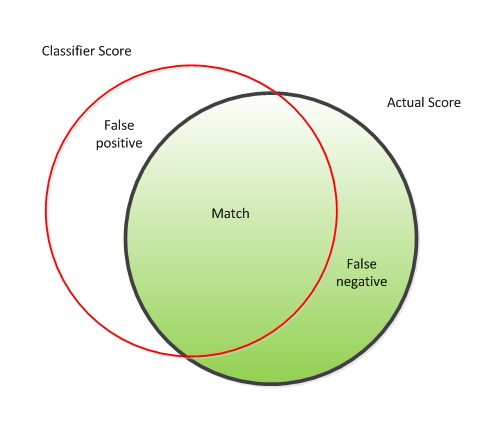
\includegraphics[scale=0.5]{figures/SingleAlgoScore}
	\caption{Variation between how a single algorithm might score an article comparison, and how the actual score should be\cite{Slides}.}
\end{figure}

The essential thing in this, is to ensure that the various algorithms works in different ways. If one were to use many algorithms that all focused on the same way of doing text comparisons, the results would not provide that broad image of scores that is wanted for a more accurate score representation.

\begin{figure}
	\centering
	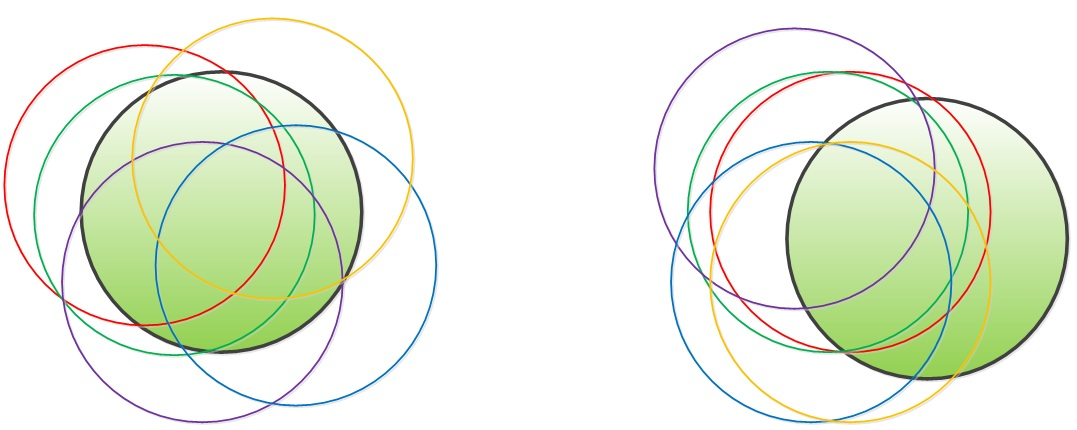
\includegraphics[scale=0.3]{figures/MultipleAlgoScores}
	\caption{\textbf{Left:} A balanced score, obtained by using several algorithm with different focus areas. \textbf{Right:} An unbalanced score, obtained by using several algorithms with the same focus area\cite{Slides}.}
\end{figure}

The idea is that the algorithms should do 99.9\% of the work in identifying article duplicates, and then have the  last 0.1\% be verified by humans. This is already how things are working at Infomedia, but only with one algorithm at the moment. My work will the be the first algorithm to do a check of the work done by the already implemented algorithm. This will hopefully narrow the field of possible article duplicates that has to be verified by human eyes.

The system would then ideally work as follows.

\begin{figure}[h]
	\centering
	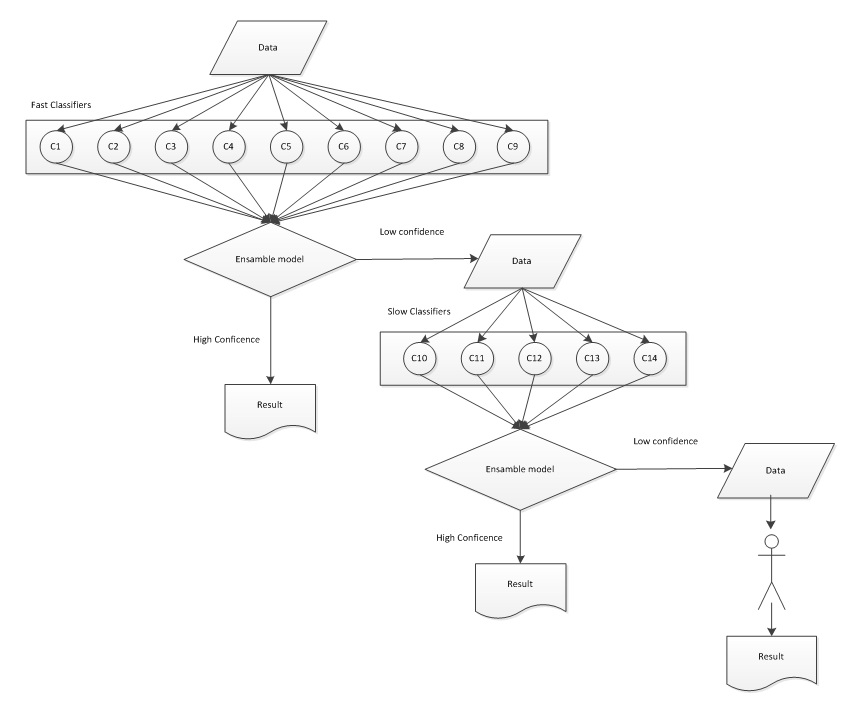
\includegraphics[scale=0.5]{figures/SystemArchitecture}
	\caption{System Architecture, with many algorithms doing text analysis\cite{Slides}.}
	\label{Architecture}
\end{figure}

When data (articles) arrives in the inflow, a number of fast algorithms would then do the rough split of the comparisons. All of these comparisons would then receive scores, that would then be evaluated through the ensemble model. If the scores leaves no doubt (is over a given threshold) that the article comparison is a match, the comparison would stored as a match. If the scores of the comparisons leaves some degree of doubt as to whether a comparison is a match or not (the scores being between a set of thresholds), the comparisons are then passed on to the slower algorithms, that then in turn would evaluate the comparisons. If these algorithms find that the comparison is a match, it would be stored as such. If there is still some doubt to whether it is a match or not, the articles would then finally be sent for human evaluation. 
The task of my thesis is to create a secondary algorithm (one of the slower ones) to evaluate the results given from the faster (and already implemented) algorithm.

\section{Algorithms Used}

\textbf{Term Frequency - Inverse Document Frequency\cite{WikiTFIDF} (Cosine)}, generates a vector from each document. \textbf{I will not cover this algorithm in detail, as I have not done any work on it, only used some of the methods in it for my thesis.} This is the algorithm already implemented in the inflow today (a modified version of it, that is based on the Vector Space Model\footnote{\url{http://en.wikipedia.org/wiki/Vector_space_model}}). Each word in every article is added to a \textit{word map} which contains all the words of all articles in the corpus being checked (which also is used to create the document vector). The word map is used to generate a weight of each word (a word occurring in many articles will have less weight than a word that is only present in a few articles). Each word generates a bit of the articles total vector, a word that occurs in all documents will have a very short vector, a more rare word will have a longer (and therefore weigh heavier) in the article vector.

Once the word map is created, the articles are then scored. The way that this is done, is that the algorithm compares two article's vectors with each other and then returns a score based on the cosine angle between the two article vectors. This is done one article comparison at a time (although done with parallel coding to speed up the process). As the word map is generated each time the algorithm is run, the word map can (and probably will) differ from each run (if the corpus of articles are being changed). Infomedia is therefore talking about implementing this bit differently, and building a constant word map, that only gets updated with each run, not overwritten. This will ensure that common words will always have a short vector.

The algorithm then returns a list of article comparisons (based on a threshold set by the user), with article ID\footnote{Each article has their own unique ID.} and scores. So each comparison has the ID of \textit{"article 1"} and \textit{"article 2"} and their score (the angle between the two vectors, in a multidimensional universe). The closer the score is to the value 1.0 the more similar are two articles. A score of 0.0 indicates that two articles has nothing in common (according to this algorithm, I will discuss this point in the next paragraph), whereas a score of 1.0 indicates two perfectly identical articles (according to this algorithm). This algorithm and it has a good O-notation (O(log N)).

\textbf{Problem:} \label{CosineProblem} This string comparison is very sensitive to articles containing many of the same words, for instance "A man walks his dog in the park" and "A dog walks his man in the park" would result in returning a cosine value of 1.0, due to the way the algorithm works. The two strings are clearly different, but the words in each string is the same, therefore the Cosine algorithm will find them to be identical. This problem is very unlikely to yield false positives.

\textbf{Longest Common Substring (LCS)}, compares documents in pairs. A general implementation would be to have a list of documents and then compare a document to every other document in the list. The algorithm will then return the length of the longest common substring. By default the LCS algorithm\cite{WikiLCS} checks the contents of a string character by character against another string. When initialized, the algorithm creates an double array and each time a match is found (when two identical characters are found ('a' and 'a' for instance)) the algorithm marks that in the array by adding a number. It then checks if this substring is longer than what has previous been found, if so, it discards the old substring and keeps the newly found.

\begin{figure}[h]
	\centering
	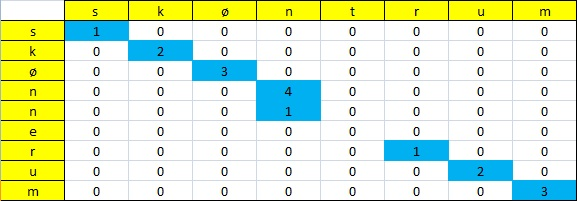
\includegraphics[scale=0.75]{figures/LcsExplained}
	\caption{An example of how two words are compared in LCS. The fields in yellow are the two words broken into characters ('Skøntrum' and 'Skønnerum'). The fields in blue indicates when LCS finds a match, the number indicates the length of the substring. In this case, LCS finds three sub strings:'skøn', 'n' and 'rum', the longest of the three is the first, and this will be the result that LCS returns to the user. }
	\label{LcsExplained}
\end{figure}

I will use the basic implementation of this algorithm in my thesis, I will then try and modify it to work better in context with finding article duplicates, instead of just the longest common substring.

\textbf{Problem:} This algorithm is very prone to fail in cases where there have been made alterations to the article in question. A word change in the middle of one of two otherwise identical articles will result in a ~50 \% match. If the article in question have been obfuscated with many changed words, the LCS will be extremely short. This is a high risk problem, as article duplication will often involve changing words. This algorithm is also substantially slower than the Cosine algorithm, having an O-notation of O(n*m). Ideally this algorithm is therefore best used on a selection of articles, rather than on the entire corpus.


\section{Optimizing Performance}
\subsection{Stop Words}
Stop word\footnote{\url{http://en.wikipedia.org/wiki/Stop_words}} removal would improve running time (performance) of both algorithms, and would pose little threat of causing either algorithm to fail (finding false positives). The exception to this could be very short articles (like breaking news articles\footnote{Breaking News articles is a thing of the 2000s. With the spread of media onto the Internet, an article is no longer a static printed piece of news in a paper. News can be published instantly on the web, and then updated as information are received. How ever, Breaking News articles can still be printed in the paper article with only little text attached to it.}), that only contains common words, like "Man walks away". Depending on the stop word list, this article could end up being \textit{null\footnote{An article with no text data.}}.
We can safely (with respects to the previously addressed problem) remove stop words, as they don't provide any \textit{semantic\footnote{\url{http://en.wikipedia.org/wiki/Semantics}}} value to the text.

\subsubsection{Cosine}
For the cosine algorithm removal of stop words would improve performance, by reducing the size of the \textit{Magnitude Vector}. 

\subsubsection{LCS}
In regards to the LCS algorithm, the performance would also be improved, as the algorithm wouldn't need to traverse as many characters. This would reduce the length of the longest common substring, but it would be unlikely that it would affect the outcome of the algorithm, as stop words are rarely changed when duplicating articles.

\subsection{Stemming}
\textit{Stemming}\footnote{\url{http://en.wikipedia.org/wiki/Stemming}} Stemming is the act of conjugating a word to the base form (Danish:\textit{'Grundform'}). It is done in order to reduce the amount of noise in a text. Words will then be conjugated and instead of having the same word represented several time in different conjugations they will all be noted as the same word. Stemming does not ruin the semantic content of the text.

\subsubsection{Cosine}
Stemming improves the performance of the cosine algorithm as this will reduce the number of words in the \textit{vector space}. As words would be reduced to their base form (Danish:\textit{Grundform}), words used several times, but with different endings would be counted as the same word. When using weighed evaluation this would actually improve performance to some extend. It can have a slight impact of the Cosine algorithm. This is because that without stemming the same word can occur several times in a text in different conjugations, and thus each conjugation would have a larger vector than when the conjugations are all counted as the same word. This impact will be minimal because the rare words are still occurring less often than normal words (stop words).

\subsubsection{LCS}
Stemming would not improve the performance of the LCS algorithm by much. As this algorithm matches characters one by one, it would make little difference if the words are stemmed or not. As the 'Grundform' is the shortest form of a word in Danish, it will make a slight difference, but this is hardly worth noting.

\section{Semaphore Tagging}
Another way of finding duplicates is by looking at each articles semaphore tags. When Infomedia receives articles in the inflow, these articles are enriched with \textit{Semaphore Tags}\footnote{Semaphore tags are tags that describes the contents of the article, an article about financial fraud would contain the tag \textit{Economic Crime}. These tags are created by the Infomedia Ontology (\url{http://en.wikipedia.org/wiki/Ontology_(information_science)}) team. They are creating rules for when a certain word (or words) appear in certain context, then an article will be tagged with a certain semaphore tag.}. A tag also has relations to other tags. A politician would be tagged with politics, political party, other people in politics that are in some way associated with that person. The tag is also enriched with a score, that is based on the relevance for that tag in that given article. So if a politician is the main focus of an article, the name of that politician is high than if the article deals with something that the politician only have a remote connection to. Each article then gets a number of tags based on what terms are found in the article. A way of finding article duplicates could be through creating an algorithm that would check a pair of articles with their respective semaphore tags.

\subsection{Cons to Semaphore}
As these tags are more of a general indicator to an articles' contents than an actual text matching algorithm, it will provide very little value as a stand alone implementation. Each article will only contain tags for the terms, for which the ontology team has created semantic rules for. If 100 articles all contained various doings of a minister (picking up the children, going to meetings, being involved in a crisis) many of the same tags would be present in the 100 articles, this could be the ministers name, political party and other general tags that are linked to this minister. It would therefore be hard to decipher much information that could truly and uniquely link two articles together just by doing this. However this could be used to enhance another algorithm (for instance one of the two mentioned above). If the articles compared contains the same tags, they are likely to have some sort of relevance to each other, and if the tags also have matching scores, that would strengthen the possibility of a match. I will not look any further into implementing this algorithm in this thesis, as this approach is difficult in providing a definite result.

\section{Text Preparation}
\label{TextPrep}
To reduce the chance of the algorithms failing in detecting duplicates, the text should be 'normalized'. As there are quite a few pitfalls in text analysis, one should try and take as many precautions as possible. A common source of error is common spelling errors, I will not check my article for spelling errors. These can have a rather big impact on the LCS algorithm. However as all text editors today have spell checking, this will be a tiny error source.

As the focus of this thesis have been on proving the thesis statement, there has been done no text preparation other than what is already implemented.

Another problem with text analysis is localized spelling. An example of this can be the Swedish town of Malmö. The issue here being the 'ö' letter which is in the Swedish alphabet. This town's name can be spelled in a few different ways.


\begin{itemize}
\item Malmö (Swedish spelling)
\item Malmø (Danish and Norwegian spelling)
\item Malmo (English spelling)
\item Malmoe (Phonetic spelling of the 'ö' character)
\end{itemize}

The same article could be in different newspapers, but with different spelling of the word. All words, or rather words containing special characters (non English characters) should therefore be normalized. In this case, the character 'ö' could be normalized into the letter 'o'. The phonetic spelling of the 'ö' character is highly unlikely to occur, as the normalized way of spelling 'Malmö' in languages without the 'ö' vowel, would be the third option. There is a lot of issues in this regard. This could be words or characters in a non Latin alphabet (Cyrillic, Arabic, Greek letters used in SI references or others). For this thesis, there is few non Danish texts or words in the test corpus, so it will have little influence. I will in this thesis not normalize text, but accept that minor deviance in scores can occur due to this.

Another good choice in text preparations is to lower case and remove all non alpha numerical characters. This can be advantageous for instance when looking at the name of the current Danish prime minister, Helle Thorning-Schmidt. As the hyphen can often be forgotten the last name can easily be misspelled. Removing the hyphen and replacing it with a blank space character would improve the accuracy of the algorithms. 

Stemming is another good way of normalizing text, I have already covered this topic in a previous section, and will not cover this more in detail here. 

Stop words will reduce the number of words in an article, and with less words, there are less error margin in terms of spelling errors, also less words in the article text means less words that has to be analysed. As stop words have little meaning when trying to figure out if two articles match, it is a good idea to remove these in order to improve performance. 

Unfortunately due to the time limit of this thesis, I will not be able to look into any of text the preparations mentioned, but wanted to describe what should be kept in mind, when implementing this project into Infomedia's inflow.

Finally it is important that all files are stored with the same encoding\footnote{\url{http://en.wikipedia.org/wiki/Character_encoding}}, as different encoding could cause havoc in the systems ability to read the text in the files. This is already done in the system, so I will not worry about this factor in my thesis.

\section{Technology}
As the inflow system at Infomedia is created in C$^\sharp$, it is the easy (and logical) choice to create my work in C$^\sharp$ as well. This would help integrating my work into the existing systems without too much trouble. I am using Visual Studio 2013 and .NET version 4.5 for my code development, which is provided to me by Infomedia. I am using Infomedias Team Foundation Server (TFS) for version control. 








                               	%Chapter 3
\chapter{Implementation}

This chapter deals with the description of implementing and modifying the LCS.

For this thesis there was created a test project in the Infomedia TFS where I could do my work. This was so that I would not mess up Infomedia's inflow while trying to make the algorithms work correctly.

First off the Cosine algorithm was implemented in said test project, and then the basic implementation of LCS was implemented.

Then the basic LCS algorithm was implemented in the project, to be used for further development.

\lstset{style=sharpc}
\begin{lstlisting}[caption=Basic LCS implementation in C$^\sharp$, captionpos=b]

public int LongestCommonSubstring(string str1,
	 string str2)
{
    if (String.IsNullOrEmpty(str1) 
    	|| String.IsNullOrEmpty(str2))
    return 0;
	
	int[,] num = new int[str1.Length, str2.Length];
	int maxlen = 0;

    for (int i = 0; i < str1.Length; i++)
  	{
    	for (int j = 0; j < str2.Length; j++)
        {
        	if (str1[i] != str2[j])
            	num[i, j] = 0;
            else
            {
            	if ((i == 0) || (j == 0))
                	num[i, j] = 1;
                else
                    num[i, j] = 1 + num[i - 1, j - 1];

                    if (num[i, j] > maxlen)
                    {
                    	maxlen = num[i, j];
                  	}
           	}
     	}
	}
    return maxlen;
}

\end{lstlisting}

The LCS works by taking in two strings as arguments and then comparing them character by character (see Figure 3.4). This works really well for finding substrings that can have been obfuscated in long lines of text. How ever in this thesis, the main objective is to find substrings of plain words rather than finding bits and pieces.

When comparing two articles with the LCS, the algorithm finds a lot of substrings, but only keeps the longest by default
\begin{figure}
	\centering
	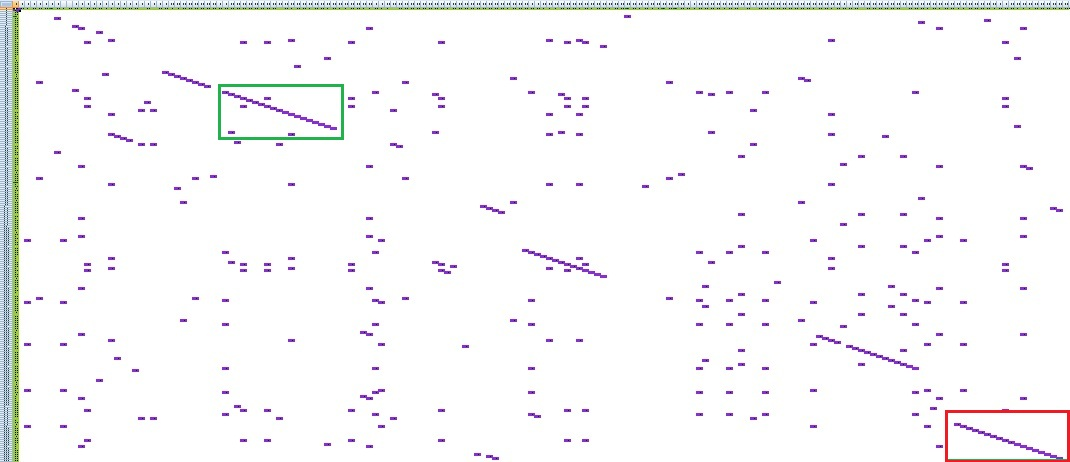
\includegraphics[scale=0.4]{figures/LcsExample}
	\caption{Diagram showing the result of two article being compared by using LCS. See Appendix A.1 for bigger image. The green and red boxes indicates longest common substrings found.}
	\label{LcsEx}
\end{figure}

The green rows seen in Figure ~\ref{LcsEx} is an article (one article along the y-axis and one along the x-axis) split into words (in the basic implementation the articles would be split in characters as seen in figure 3.4, this figure is from the updated version of LCS). All the purple boxes indicates where a match has been found, a diagonal line indicates a row of matches. The longest one would be the \textit{'Longest Common Substring'} and the length of that would be returned by the algorithm. In the example from Figure ~\ref{LcsEx} there are two substrings of equal length (each having a length of 19 words (in the basic LCS the length would the number of characters, including white spaces)), how ever as LCS only returns the length of a single longest common substring (the longest found) and the second one (marked in the red box) is same length, LCS returns the length of the first (marked in the green box) substring. Again, as this example is made out of words rather than characters, the result could vary in case of counting actual characters, but for demonstration purposes the figure explains the idea.

In the case of a perfect match (require both articles to be of the exact same length). A line along the diagonal will be drawn.

\begin{figure}
	\centering
	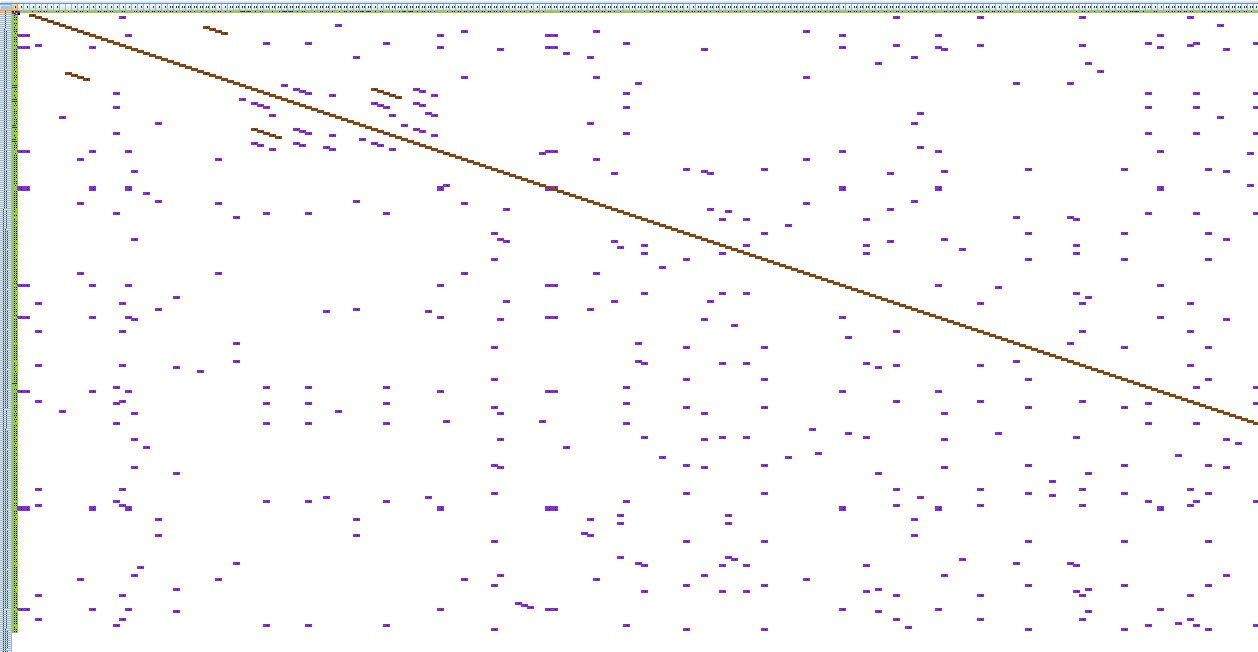
\includegraphics[scale=0.4]{figures/PerfectMatch}
	\caption{Diagram showing a part of an almost perfect match (the article along the y-axis is slightly longer than the article along the x-axis)}
	\label{Match}
\end{figure}

In Figure ~\ref{Match} there is two article that are almost 100\% identical. One of the articles ~\cite{JV1} is slightly shorter than the other article \cite{Lemvig1}. The on line content of the second article is protected by a payment wall, the article content can be found in Appendix B.

The next step was to modify the LCS algorithm to make suit the needs of this thesis. When looking at article duplicates, it makes more sense to look for entire words rather than single characters. This is because when an article is duplicated, any obfuscation or alteration would be done by cutting out sections of the article or moving sections around or adding new sections.



							%Chapter 4, Implementation
\chapter{Test}

This chapter describes the tests that was done to make sure the implementation of LCS was working correctly. Also various tests was done on the test corpus using the Cosine algorithm. 

During the test segment, there was a focus on mainly four sources (their article content), those being \textit{Berlingske Tidne (BERL), Politiken (POL), JV.dk (JV) and \\* http://folkebladetlemvig.dk/ (FL)}. There is various reasons for picking those four. Berlingske Tidne and Politiken are nation wide papers, and some of the most read in Denmark. As such, they have big budgets, big staffs and can afford doing a lot of journalistic work of their own. They could often deal with the same topics, can use the same news agencies (such as Reuters), but would often have a lot of unique material (at least that is the theory to be tested). jv.dk and folkebladetlemvig.dk are both local papers, meaning they they are only published in parts of the country. This means they to a larger extend deals with local happenings and news. They will have less focus on international material. As a small paper they will have small budgets, smaller staff and may not have the journalistic manpower to do much ground breaking, in-depth journalistic work. Also these papers are often distributed freely (their on line content may be protected by a payment wall) in the local area, and as such, their main revenue is adds sales. These adds will take up a lot of space in these papers, allowing for less news articles that in the bigger news papers. Finally a reason for picking these two sources in particular is that they are both owned by Belingske Media (who also owns Berlingske Tidne), and they do therefore make a good case for testing how much material is shared between media.

After doing the various implementations of the algorithms, testing was made to verify the correctness of these implementations. This interweaves with the sections of the previous chapter.

\section{Test of the basic LCS}

\begin{figure}
	\centering
	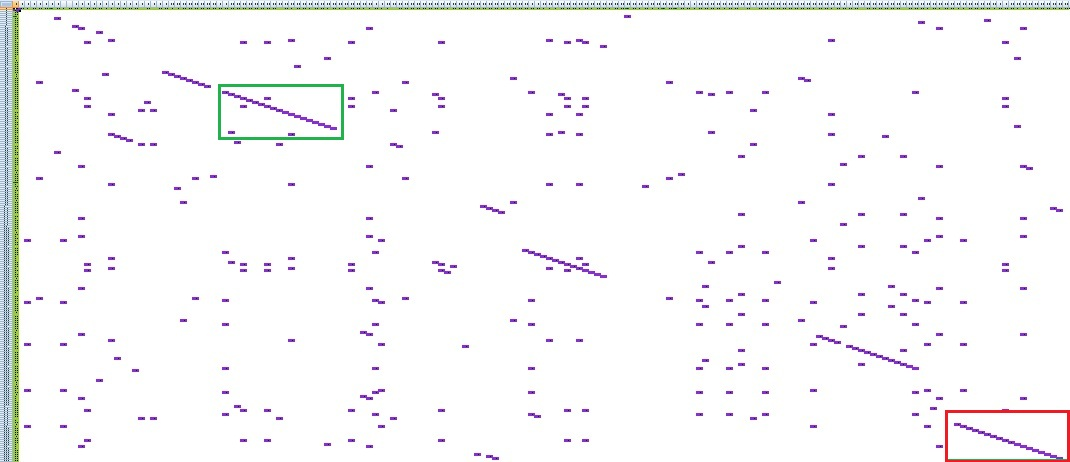
\includegraphics[scale=0.4]{figures/LcsExample}
	\caption{Diagram showing the result of two articles being compared by using LCS, and plotted in Excels. See Appendix A.1 for bigger image. The green and red boxes indicates longest common substrings found.}
	\label{LcsEx}
\end{figure}

As the final stage of the system implemented, to deal with the article duplication, there is a part that deals with post processing (see figure ~\ref{Dataflow}). This post processing mainly deals with setting up data in reader friendly way. This involves printing results to an Excel spreadsheet. Plotting the results of the LCS to a spreadsheet helps to illustrate how LCS works, and what results are being found. 

An example of this type of plot can be seen in figure~\ref{LcsEx}. The leftmost column (in green) is one article split into words, the topmost row (also in green) is another article split into words (in the basic LCS implementation the articles would be split in characters as seen in figure ~\ref{LcsExplained}). All the purple boxes indicates where a match has been found, a diagonal line indicates a row (substring) of matches. The longest one would be the \textit{'Longest Common Substring'} and the length of that would be returned by the algorithm. In the example from Figure ~\ref{LcsEx} there are two substrings of equal length (each having a length of 19 words (in the basic LCS the length would the number of characters, including white spaces)), how ever as LCS only returns the length of a single longest common substring (the longest found) and the second one (marked in the red box) is same length, LCS returns the length of the first (marked in the green box) substring. Again, as this example is made out of words rather than characters, the result could vary in case of counting actual characters, but for demonstration purposes the figure explains the idea.

In the case of a perfect match (require both articles to be of the exact same length). A line along the diagonal will be drawn. Of course the nature of representing all text in a horizontal way, distorts the image somewhat, as this makes the x-axis seem shorter than the y-axis even though the two might be of equal length. 

So, what does this image tell us? Well, for starters it shows us how LCS works. It helps us see how many words the two articles have in common, and it also helps us get an overview of how similar the two articles are, in terms of being duplicated. This was the goal of implementing the LCS in the first place.

\begin{figure}
	\centering
	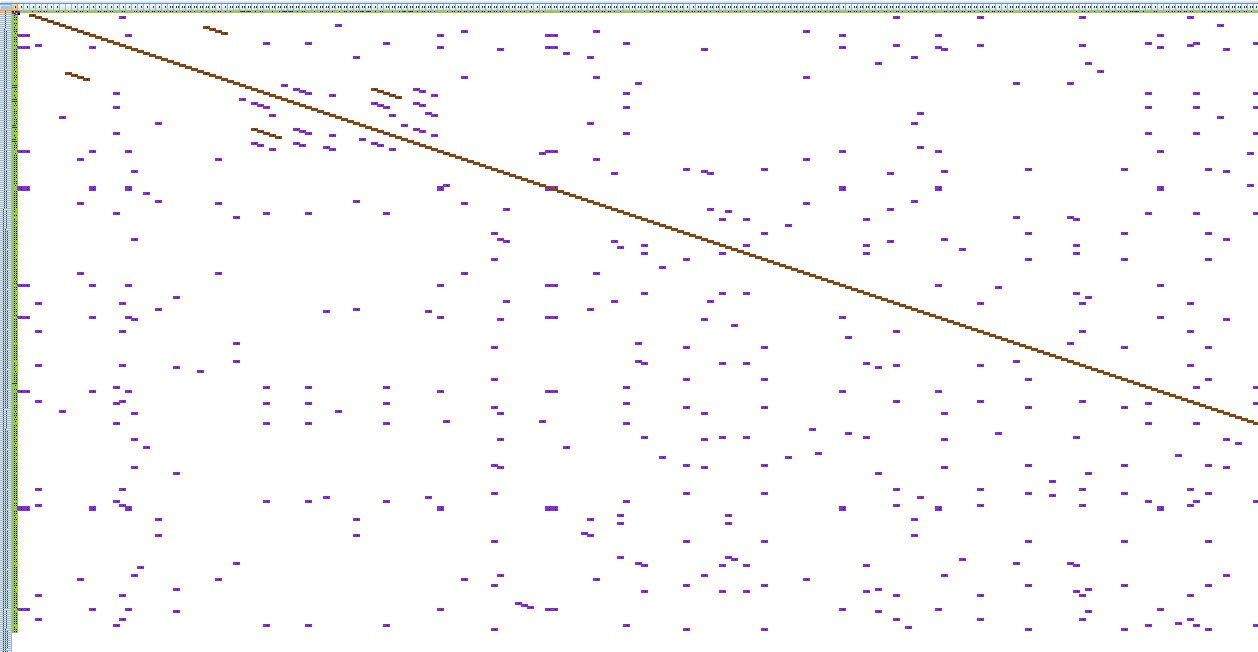
\includegraphics[scale=0.35]{figures/PerfectMatch}
	\caption{Diagram showing a part of an almost perfect match (the article along the y-axis is slightly longer than the article along the x-axis). The long brown diagonal line indicates the longest common substring found.}
	\label{Match}
\end{figure}

In Figure ~\ref{Match} there is two articles that are almost 100\% identical, the articles are from JV and FL. One of the articles ~\cite{JV1} is slightly shorter than the other article ~\cite{Lemvig1}. The on line content of the second article is protected by a payment wall, the article content can be found in Appendix B ~\ref{Levmig1:text}.
What is a added bonus of these two articles is that not only are they clearly duplicates, they are also written by the same author, \textit{Johan Winther}, who happens to be a journalist working for BERL\footnote{\url{http://www.b.dk/redaktionen/johan-winther}} as per 2014-05-22. This supports the thesis that the local papers, are fed news from their owning papers, to print in their own papers. This can be out of various reasons, one could be that the owning paper would have covered a story of nation wide importance, but with a special local importance. In this case, the articles deals with the company Danfoss, which is a big company in southern Jutland, and therefore has a big significance for the ares which is covered by the two local papers (JV covers southern Jutland, and FL covers the mid-west-northern part of Jutland).

\section{Test of the Modified LCS}

Once the modified version of LCS was implemented, the post processing underwent some changes to support this. The Excel printing was modified to colour the longest common substrings found, that was longer than the given threshold. All substrings that match that criteria is coloured in brown in the following. After doing some testing with the threshold, a threshold of four was selected. That value seemed to include most important sentences in terms of finding duplicates, without including too much text. Whether we remove stop words or not, should be considered when setting the threshold. Stop words are the easiest to remove or alter when modifying text, as they add little meaning to the overall topic of the text. With efficient stop removal, only key (or more significant) words will remain. These are in much higher degree a pointer to the similarity of two texts.

\begin{figure}
	\centering
	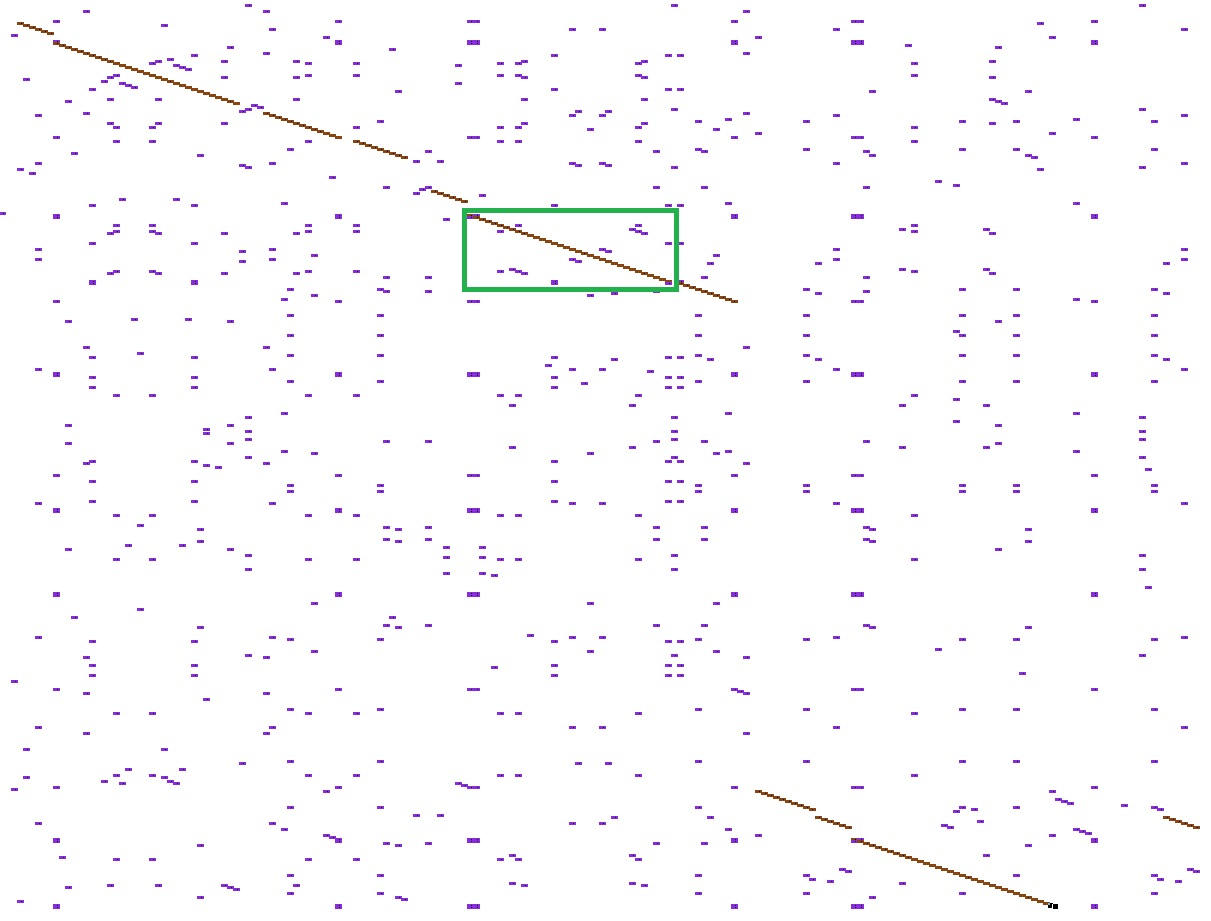
\includegraphics[scale=0.35]{figures/SubstringCollection}
	\caption{The result of having a collection of substrings (this being a part of the full image - the spreadsheet can be seen in the file "Lcs perfect match.xlsx"). All substrings with a minimum length equal or grater to the threshold, have been coloured brown. All substrings that is short than this, is coloured in purple. If only the longest substring had been returned as the result, only the substring (marked by the brown line) in the green box would have been returned.}
	\label{SubstringsEx}
\end{figure}

As seen in figure ~\ref{SubstringsEx} the addition of substring collection significantly alters the result from what we would have gotten, had we only been using the basic LCS implementation. Judging from this diagram the two articles obviously have a lot in common. To tell if the article really have something in common it is needed to take a look at their content. The best way of doing this is by reading it the old fashion way, with your own eyes.  All of the verification done in a prototype is expected to be done this way, once the users are satisfied (through repeated manual verification) that no or only very few errors would bypass the algorithms, then the verification would be left to the algorithms (as per figure ~\ref{Architecture}).

\section{Fractile Distribution of Corpus}
The way that Consine is implemented in the inflow now, is by scoring article comparisons based on the angle between the article's vectors. This score then indicates (to some extend) how alike two articles are. The score ranges from 0.0 to 1.0. In the inflow, Infomedia simply stores all comparisons with a score above 0.6, these articles can then be verified (this is where LCS will come in handy). For this thesis however, we will compare all articles and then use the LCS on those with a Cosine score above a certain threshold. A Cosine score above 0.9 indicates, with a high degree of certainty, that the two articles being compared are practical identical (there can be modifications to this statement, will be discussed later). A certain Cosine score would therefore qualify for a comparison being automatically accepted as identical, articles below that score and down to a lower threshold would then have to controlled by human eyes. So we would like the LCS to do some of work for the humans by further cutting down the field of possible duplicates. The idea of the Cosine algorithm doing the initial splitting of article comparisons and then letting the somewhat slower LCS algorithm look into the comparisons which are uncertain in relation to being duplicates raises the following question, how many article comparisons are we looking at? For this a test of the test corpus would be made in order to give a visual representation of the task ahead.

Before setting out on the task of comparing all articles in the test corpus, a minor test made initially. The Cosine algorithm put to work with scoring all articles from BERL and POL sources in the test corpus, storing the results in fractiles(by intervals of 0.1), and then printing them to an Excel spreadsheet.

\begin{figure}
	\centering
	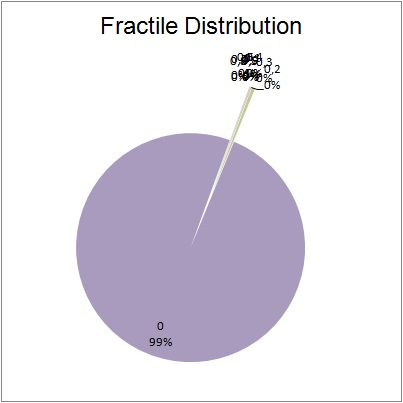
\includegraphics[scale=1.0]{figures/FractileNoise}
	\caption{The result of running Cosine on all articles in the BERL and POL sources (File: "fractile noise.xlsx").}
	\label{FractileNoise}
\end{figure}

As seen in figure ~\ref{FractileNoise}, the vast majority of the article comparison are in the lowest fractile (0.0-0.1 Cosine score), and makes it really hard to use the pie chart for any sort of informative source. The scores are distributed as seen in table ~\ref{TestFractile}.

\begin{table}
\begin{center}
	\begin{tabular}{l | r}
		Cosine Score (x) & Number of Comparisons\\ \hline
		x $\leq$ 1.0 $\bigwedge$ x $\geq$ 0.9 & 2 \\ \hline
		x < 0.9 $\bigwedge$ x $\geq$ 0.8 & 1 \\ \hline
		x < 0.8 $\bigwedge$ x $\geq$ 0.7 & 0 \\ \hline
		x < 0.7 $\bigwedge$ x $\geq$ 0.6 & 1 \\ \hline
		x < 0.6 $\bigwedge$ x $\geq$ 0.5 & 2 \\ \hline
		x < 0.5 $\bigwedge$ x $\geq$ 0.4 & 8 \\ \hline
		x < 0.4 $\bigwedge$ x $\geq$ 0.3 & 9 \\ \hline
		x < 0.3 $\bigwedge$ x $\geq$ 0.2 & 17 \\ \hline
		x < 0.2 $\bigwedge$ x $\geq$ 0.1 & 98 \\ \hline
		x < 0.1 $\bigwedge$ x $\geq$ 0.0 & 21608 \\ \hline	
		Total Comparisons & 21746 \\ \hline
	\end{tabular}
\end{center}
\caption{Fractile distribution of article comparisons for BERL and POL.}\label{TestFractile}
\end{table}

So in order to get a more informative view, removing the lowest fractile (comparisons scoring below 0.1 with the Cosine algorithm) will provide a better view (see figure ~\ref{NoNoise}). Please note that the value given in the various of the sections of the pie chart, is the minimum value of the fractile in question and percentage of comparisons in that fractile. The fractile named '0,9' is the fractile containing all comparisons that scored between 1.0 and 0.9(included).

\begin{figure}
	\centering
	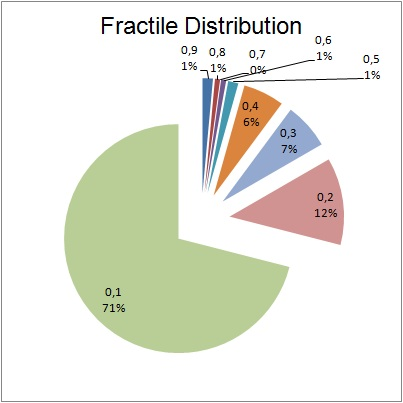
\includegraphics[scale=1.0]{figures/FractileNoNoise}
	\caption{Fractile distribution (BERL and POL articles) with the comparisons scoring lower than 0.1 in the Cosine comparison removed.}
	\label{NoNoise}
\end{figure}

To double check the test result, and also to test the thesis that JV and FL do share a significant number of articles, a fractile distribution graph was made for those two sources ~\ref{JVFLFractile}.

\begin{figure}
	\centering
	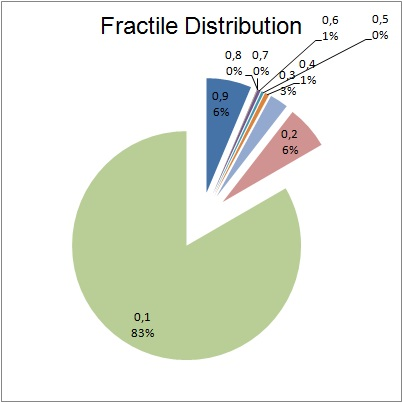
\includegraphics[scale=1.0]{figures/JVFLFractile}
	\caption{Fractile distribution (JV and FL articles) with the comparisons scoring lower than 0.1 in the Cosine comparison removed.}
	\label{JVFLFractile}
\end{figure}

\begin{table}
\begin{center}
	\begin{tabular}{l | r}
		Cosine Score (x) & Number of Comparisons\\ \hline
		x $\leq$ 1.0 $\bigwedge$ x $\geq$ 0.9 & 102 \\ \hline
		x < 0.9 $\bigwedge$ x $\geq$ 0.8 & 1 \\ \hline
		x < 0.8 $\bigwedge$ x $\geq$ 0.7 & 1 \\ \hline
		x < 0.7 $\bigwedge$ x $\geq$ 0.6 & 7 \\ \hline
		x < 0.6 $\bigwedge$ x $\geq$ 0.5 & 6 \\ \hline
		x < 0.5 $\bigwedge$ x $\geq$ 0.4 & 10 \\ \hline
		x < 0.4 $\bigwedge$ x $\geq$ 0.3 & 42 \\ \hline
		x < 0.3 $\bigwedge$ x $\geq$ 0.2 & 99 \\ \hline
		x < 0.2 $\bigwedge$ x $\geq$ 0.1 & 1342 \\ \hline
		x < 0.1 $\bigwedge$ x $\geq$ 0.0 & 53017 \\ \hline	
		Total Comparisons & 54627 \\ \hline
	\end{tabular}
\end{center}
\caption{Fractile distribution of article comparisons for JV and FL.}\label{Test2Fractile}
\end{table}


Once again we see a large amount of comparisons in the 0.1-0.2 fractile ~\ref{JVFLFractile}, it being a great deal bigger (83\% versus the 71\% in figure ~\ref{NoNoise} in the 0.1-0.2 fractile). We do however also see a bigger amount of comparisons in the top fractile (0.9-1.0) which would indicate that these two sources actually share quite a few articles, and also have more articles in common than BERL and POL.

As a final test, to get the big picture of the task ahead, a test was performed for all articles in the test corpus (File: "symmetric all files fractiles.xlsx"). When running the Cosine algorithm, it is given three parameters the two first being the files to be compared, the third being a list that will contains the comparison score along with the articles information. Cosine starts with making a check of the two file sets, if they are the same, it will do a triangle comparison. This means we only have to check half the number of possible comparisons - minus the diagonal. This is handy if we want to do a comparison on a single set of articles. If you want to compare the articles two days (or some other time frame), the algorithm will do an asymmetrical comparison, meaning that all possible comparisons are made - minus the diagonal, as checking an article with itself is trivial.

\begin{figure}
	\centering
	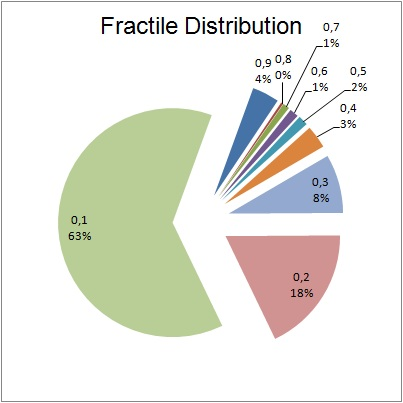
\includegraphics[scale=1.0]{figures/AllFilesFractile}
	\caption{Cosine comparison of all files in the test corpus. The fractile below 0.1 have been left out, to create a better view of the comparison distribution (File: "symmetric all files fractiles.xlsx").}
	\label{Fractles}
\end{figure}


The scores of the final test are distributed as follows (the fractile below 0.1 have been included in this table, it accounts for 99\% of the total number of comparisons) in table ~\ref{AllFractiles}.

\begin{table}
\begin{center}
	\begin{tabular}{l | r}
		Cosine Score (x) & Number of Comparisons\\ \hline
		x $\leq$ 1.0 $\bigwedge$ x $\geq$ 0.9 & 61107 \\ \hline
		x < 0.9 $\bigwedge$ x $\geq$ 0.8 & 5168 \\ \hline
		x < 0.8 $\bigwedge$ x $\geq$ 0.7 & 15090 \\ \hline
		x < 0.7 $\bigwedge$ x $\geq$ 0.6 & 20443 \\ \hline
		x < 0.6 $\bigwedge$ x $\geq$ 0.5 & 22472 \\ \hline
		x < 0.5 $\bigwedge$ x $\geq$ 0.4 & 51945 \\ \hline
		x < 0.4 $\bigwedge$ x $\geq$ 0.3 & 132699 \\ \hline
		x < 0.3 $\bigwedge$ x $\geq$ 0.2 & 286529 \\ \hline
		x < 0.2 $\bigwedge$ x $\geq$ 0.1 & 1001151 \\ \hline
		x < 0.1 $\bigwedge$ x $\geq$ 0.0 & 247311986 \\ \hline	
		Total Comparisons & 248908590 \\ \hline
	\end{tabular}
\end{center}
\caption{Fractile distribution for all files compared in Cosine.} \label{AllFractiles}
\end{table}

As table ~\ref{AllFractiles} shows, there is a massive amount of comparisons in the lowest fractile (close to quarter of a billion comparisons, the total number of comparisons above that is approximately 1,6 million comparisons (1,596,604 comparisons).

After doing these test, it would seem like the various parts of the project is working as planned, and it is now time to evaluate the results produced by running the program.
										%Chapter 5, Test
\chapter{Evaluation}
This chapter deals with evaluating the results from the program when scoring article comparisons.

After having done tests to verify that the implementation of the algorithms worked correctly, it is now time to analyse the output.

\section{Scores}

The Cosine algorithm returns a score that is in fact an angle, where as the LCS algorithm returns a score that is based on the length of a string. As such these are hardly comparable in a one to one basis. If we modify the score of the LCS to not say something about the length of the substring(s), but tell us in percent how long the string is compared to the article is, it will produce a result that relates to the amount of text the two articles being compared have in common. This being said we still need to consider that the percentage value is relative to the length of the length of the article. We do therefore need to do a percentage calculation for both article's length. For better comparison of the Cosine and LCS score in the Excel graphs, the LCS percentage score is divided by 100 (even though comparing the scores is not really a decent indicator, it helps giving a better overview of the graphs).

So, a Cosine score of 1.0 means that the two article vectors are identical, same length and no angle between them. A LCS score of 1.0 means that the longest common substring's length is 100\% of the article's length. So each score will have to be evaluated on their own premisses, as a Cosine score of 0.5 is not 50\% identical. The Cosine score tells us something about how many special words that two articles have in common, where are the LCS tells us about the amount of text (substrings) that is shared between the two articles.

\section{Limiting the Number of Comparisons by Cosine Score}

As discussed in the last chapter (see section ~\ref{AllFractiles}) there is many comparisons in the lowest fractile of the article comparisons. Although dismissing them right of the bat can be seen as hasty, the chance of comparisons scoring below 0.3 having much in common would be unlikely. This is because comparisons that score very low in the Cosine algorithm either have very little in common in terms of special words (as common words will have very little impact on the vector) or the article is very short and again, with few special words (we will see an example of this later on). However, an article with no special words that is very short, is very rare and few in between. We will however see examples of such articles later on.

For the sake of proving anything in this thesis how ever, and as the chance of getting useful results from comparisons with low Cosine scores are slim and the number of comparisons having to be humanly checked are massive in numbers should we check all comparisons, I will for the rest of this thesis, disregard all comparisons with a cosine score lower than 0.3.

\section{What the Scores Tell}
First off we need to realize what the different scores is telling us on their own. The cosine score will give an indication of how similar two articles are in regards to the words being used, but will not tell us anything in regards to what the article is actually saying in regards to the structure of sentences (see section ~\ref{CosineProblem}). By it's own, Cosine will tell us more about if the comparisons have the same topic that actually the same sentences. 

The modified LCS is an indication of how big a percentage of text in relation to article length that an article have in common with another article. The LCS score will therefore tell us a lot about how much actual text a comparison shares. 

\subsection{Definition of "High Scoring"}
A lot of the results in the result sets, are subject to a lot of "gut feelings". There will be mentions of "high" score values. This is of course a relative term, because when can we truly define a score as high? For the Cosine part a high score would be 0.9 and higher. Below that we can start to see gray areas in which the score is not definite any more. When speaking of high scores in the LCS values things start to become even more fuzzy. A LCS score of 0.3 might be telling a lot in articles that is very long, but in very short articles, that score might just mean a single substring consisting of few words. The term high should in this relation be considered on a basis of the score value and the length of the article. This issue will be discussed later.

\section{Score Analysis}

In figure ~\ref{SubstringsEx} we see a part of the LCS result of two articles being compared with each other. A long each axis we have an article (topmost row and leftmost column - not visible on image). The purple squares shows where a word match have been found, and a diagonal row of coloured squares indicate several words in concession have been found. If squares are coloured in purple, it means that the substring found is too short, if the squares are in brown the substring is equal to or greater than the threshold set for accepting substrings.

In the figure we see that the two articles start off with having a lot in common, then around two thirds into figure there is a huge gap along the x-axis, but it is largely unbroken along the y axis. So if judging the result by looking at this image we can establish two things.

\begin{itemize}
\item The two articles have a lot of text in common, but the article along the x-axis is substantially longer than the article along the y-axis.
\item The article along the y-axis is an excerpt of the article along the x-axis.
\end{itemize}

So when looking at this plot, we can tell if an article comparison is a duplicate, a excerpt or if there is no real match between two articles. To validate this fully it is needed to read the article text, to make sure the combination of substrings is not just a collection of random words, that are aligned in the same way without any relation.

In the following when looking at LCS comparison of articles, they are plotted like this in Excel. 

\section{Analysis of Comparisons}
In the following is described the evaluation of the scores produced by matching the four sources (JP being matched with POL and JV being matched with FL). In this section there will be a lot of references to Excel files. These are included in the electronic version of this thesis. In the two files containing the comparisons for all articles in the source folders (File: JPPOL.xlsx and JV-Lemvig.xlsx), some of the comparisons are marked with \textit{Match}, \textit{PartialMatch}, \textit{SameContent} and \textit{LowScoreMatch}. These comparisons have been plotted in Excel as well, and they are included in their respective source folders labelled with that match name and the name of the files is the combination of the ids in the comparisons.

\subsection{JP and POL Comparison}
First off, the sources POL and JP was compared in the program. The results of this was then plotted in Excel (File: JPPOL.xlsx). The data columns are:

\begin{itemize}
\item \textbf{Left Id / Right Id:} The article Ids of the comparison. These are used to find the articles, when checking their content manually.
\item \textbf{Cosine Score:} The Cosine score for the comparison.
\item \textbf{LCS Score:} The unmodified LCS score. This is included for comparison with the modified LCS score. It is a percentage score off the longest of the two articles in the comparison.
\item \textbf{Combined Score Max:} The score from the modified LCS. This is a percentage score off the longest of the two articles in the comparison.
\item \textbf{Combined Score Min:} The score from the modified LCS. This is a percentage score off the shortest of the two articles in the comparison.
\item \textbf{Long Length:} The length of the longest article in characters.
\item \textbf{Short Length:} The length of the shortest article in characters.
\item \textbf{Match Group:} The match group the comparison have been placed into by the program (this will be explained later).
\item \textbf{Adjusted Score:} The score modification after applying score weighing (this will also be explained later).
\end{itemize}

Originally only the LCS score based off the longest article was included and used for evaluating the results. It did become clear after the first few tests, that this would not suffice. If we looked at two articles, one being substantially longer than the other, but the shortest being a 100\% excerpt of the longest, we could end up in a case where the article comparison would score very low because the LCS (and the Cosine for that matter) would be very low. We could then end up discarding this comparison as a "no match" because the scores was too low. How ever if we looked at the LCS score based off the length of the shortest article, we would get a completely different image. Then we could actually detect that the shortest article was in fact a excerpt, by seeing that it's LCS score would be 100\%. We will therefore have to look into the length of the articles as well, in order to fully say something about how much of a match a comparison is (this will be brought up again later).

Finally there are three graphs. The first is \textit{'Sample Distribution with Stopwords'}. This shows in a column diagram the comparisons different scores. As mentioned earlier we cannot compare the Cosine score with the LCS score on a one to one basis. However this does indicate something about general relations.

\begin{figure}
	\centering
	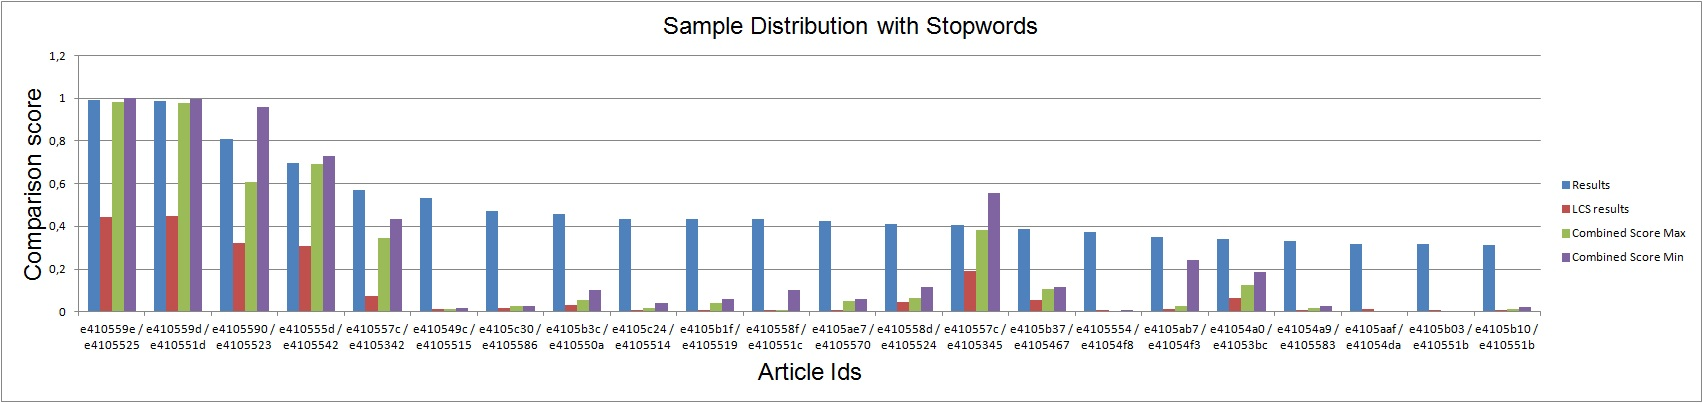
\includegraphics[scale=0.25]{figures/JPPOLScoreGraph}
	\caption{Comparison scores for the JP and POL sources (see appendix D for bigger image or File: JPPOL.xlsx).}
	\label{JPPOLScoreGraph}
\end{figure}

Figure ~\ref{JPPOLScoreGraph} shows the effect of having the modified LCS to collect all substrings longer than a given threshold. It also shows the necessity of having to evaluate the LCS score with both the length of the longest and the shortest article length as there can be quite a big difference in the scores.

Below that graph is two graphs side by side. The first shows the Cosine score plotted with the modified LCS score based off the longest article. The second graph shows the same, but this time the red dots is showing the Cosine and modified LCS score based off the shortest article.

The graphs in figure ~\ref{MaxScore} and ~\ref{MinScore} was created in order to get a better overview of how the scores was distributed. 

\begin{figure}
	\centering
	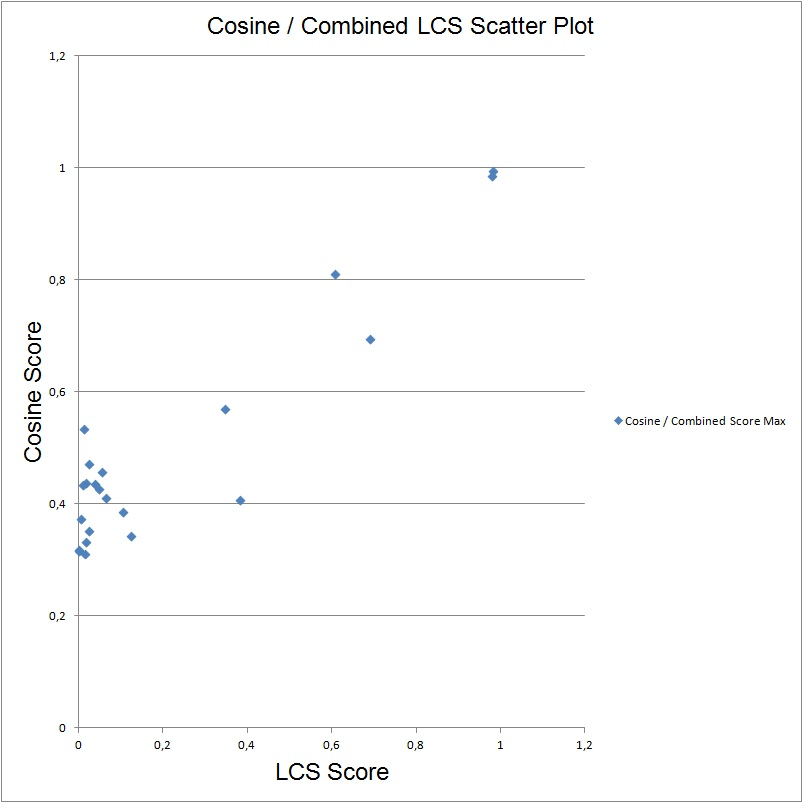
\includegraphics[scale=0.5]{figures/JPPOLCosineLCSMax}
	\caption{A plot showing the Cosine / LCS score (based of the longest article length in the comparison).}
	\label{MaxScore}
\end{figure}

\begin{figure}
	\centering
	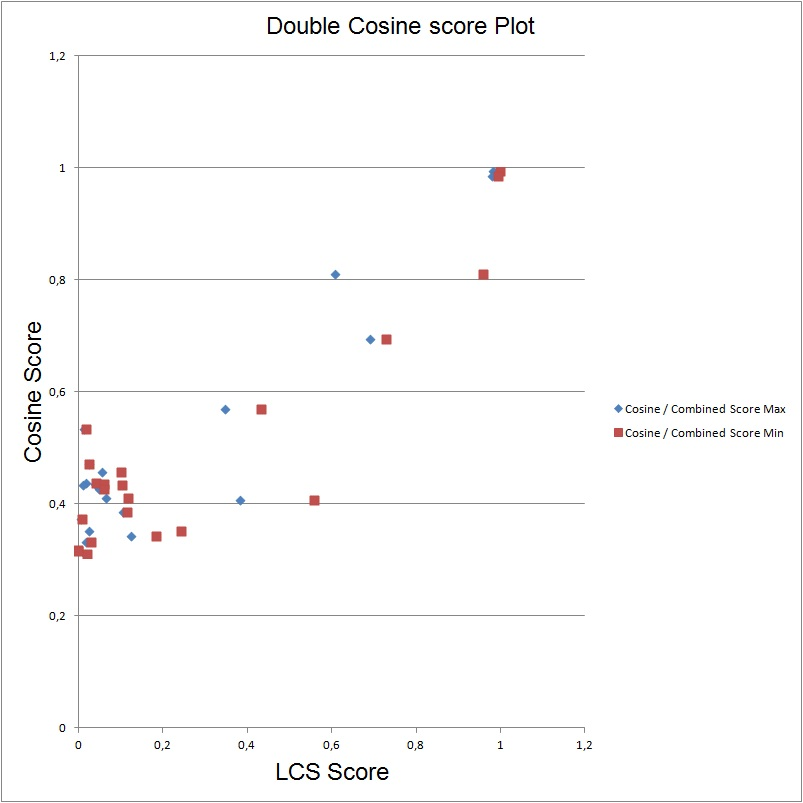
\includegraphics[scale=0.5]{figures/JPPOLCosineLCSMin}
	\caption{A plot showing the Cosine / LCS score (based off the longest article length - the blue dots) and the Cosine / LCS score (based off the shortest article length - the red squares).}
		\label{MinScore}
\end{figure}

When evaluating the figure ~\ref{JPPOLScoreGraph} we can start with looking at the first two collections of scores (comparisons \textit{e410559e / e4105525} and \textit{e410559d / e410551d}). Both comparisons have high scores in all columns. We note that the basic LCS scores around half as high as the scores for the two modified LCS scores. For the rest of this thesis I will disregard the scores produced by the basic LCS, as it holds no meaningful data when trying to find article duplicates. The length of the four articles in the comparisons is around the same length, meaning both of the LCS scores is more or less equally high.

The thesis about the algorithm scores can be now be verified. From the excel file we get the scores seen in table ~\ref{JPPOLHighScores} and table ~\ref{JPPOLSecondHighestScores}. The scores is sorted by Cosine score. 

\begin{table}
\begin{center}
	\begin{tabular}{l | r}
	Ids & e410559e / e4105525\\ \hline
	Cosine & 0.992916226\\ \hline
	Basic LCS & 0.441762865\\ \hline
	LCS (long article) & 0.981112301\\ \hline
	LCS (short article) & 0.998931646\\ \hline
	Long article length & 953\\ \hline
	Short article length & 936\\ \hline	
	\end{tabular}
\end{center}
\caption{Scores for the highest scoring article comparison when comparing JP and POL sources (File: JPPOL.xlsx). The two last LCS scores is the LCS score percentage based off the longest article, and the scored based off the shortest article.}
\label{JPPOLHighScores}
\end{table}

\begin{table}
\begin{center}
	\begin{tabular}{l | r}
	Ids & e410559d / e410551d\\ \hline
	Cosine & 0.985605299\\ \hline
	Basic LCS & 0.449531734\\ \hline
	LCS (long article) & 0.979188323\\ \hline
	LCS (short article) & 0.994714558\\ \hline
	Long article length & 961\\ \hline
	Short article length & 936\\ \hline	
	\end{tabular}
\end{center}
\caption{Scores for the second highest scoring article comparison when comparing JP and POL sources (File: JPPOL.xlsx).}
\label{JPPOLSecondHighestScores}
\end{table}

When looking at table ~\ref{JPPOLHighScores} all the algorithm scores are high, all near 1.0 (except from the basic LCS score which we disregard). The articles are of similar length and they have a length that indicates that they contain a lot of text. To begin with, we will evaluate the results by looking at the LCS plot.


\begin{figure}
	\centering
	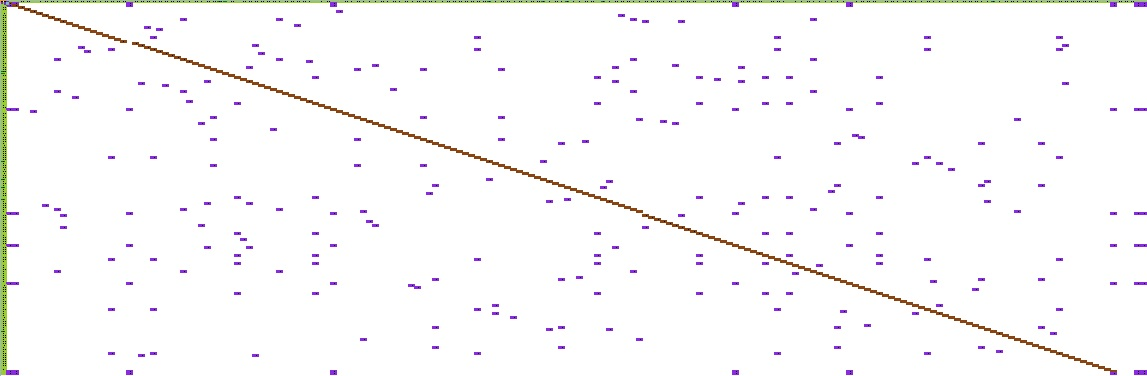
\includegraphics[scale=0.35]{figures/e410559e}
	\caption{Plot of the result of comparing article e410559e and article e4105525 using the LCS algorithm (File: e410559e-e4105525.xlsx). See appendix ~\ref{D2} for a bigger image.}
	\label{JPPOLHighestLCS}
\end{figure}

The plot ~\ref{D2} clearly shows a diagonal line going from top left towards bottom right. There are a few minor deviances along the way, which corresponds well with what the LCS score tells us, that the we are just a tiny bit away from having a 100\% perfect match. 

After the initial verification, comes the task of manually checking the content of the articles to make sure that they are in fact (almost) identical. The article text can be found in appendix ~\ref{JPPOLHighestMatch1} and appendix ~\ref{JPPOLHighstMatch2}. After reading the text it is clear that the texts are in fact identical, except from the very last sentence in the first article ~\ref{JPPOLHighestMatch1} which only contains an email, but then what about the two breaks in the middle of the comparisons? This is where the issue of text normalization becomes evident. The differences marked by the LCS is actually caused by the way the XML files containing the article text is read. In the figures ~\ref{XmlIssue1} and ~\ref{XmlIssue2} we can see that one article have a paragraph break in a sentence that the other article does not have. The way that text is being extracted by the Cosine algorithm (it is a part of the program that does the Cosine comparison that also extracts the text from the XML files, this is of course done before the comparison is made, and is a part of the system that was not implemented in this thesis), removes non alphabetic characters, in this case the punctuation. In the other article the paragraph also ends with a punctuation, but when that is removed, there is no word following the last word in the paragraph like in the other article. This means that one article will then have a white space that is not present in the other article. In order to fix this, text should be normalized in a way that makes sure that all paragraph breaks inserts a white space into the text if one is not present already. If that had been done, the LCS score would have been higher. This problem is present in a lot of the results, but is unlikely to cause a significant error source (but should be kept in mind). This problem is frequently occurring in article duplicates, as articles will be broken into paragraphs that might fit the layout of the paper, or due to other reasons.

\begin{figure}
	\centering
	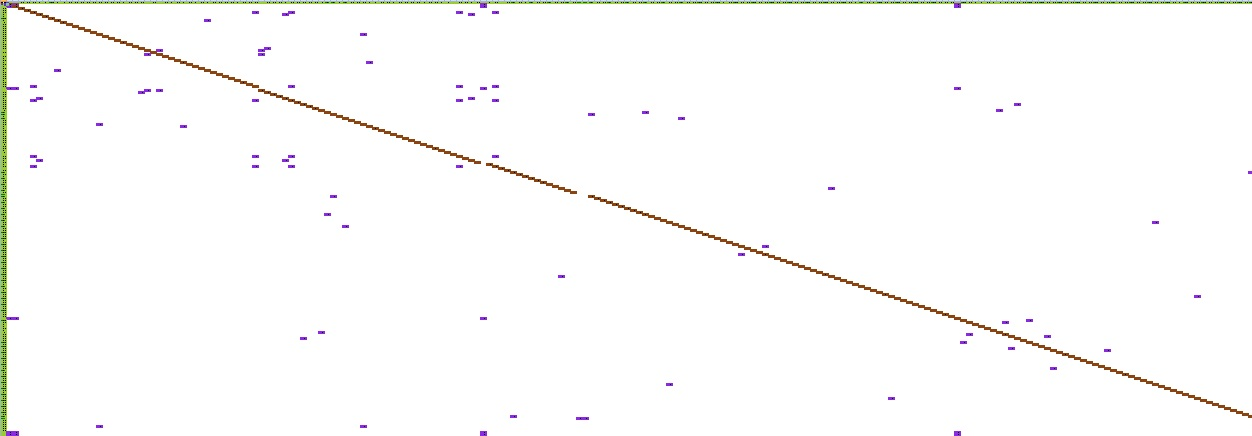
\includegraphics[scale=0.35]{figures/e410559d}
	\caption{Plot of the comparisons of articles e410559d and e410551d (File: e410559d-e410551d.xlsx)}
	\label{JPPOLSencondHighestLCS}
\end{figure}

\begin{figure}
 	\centering
 	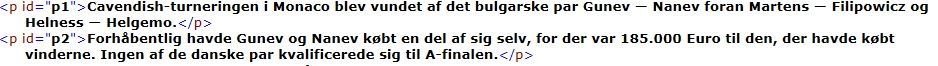
\includegraphics[scale=0.5]{figures/XmlIssue1}
 	\caption{Excerpt from the XML file containing the text found in appendix ~\ref{JPPOLHighestMatch1}.}
 	\label{XmlIssue1}
\end{figure}

\begin{figure}
	\centering
	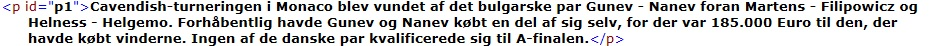
\includegraphics[scale=0.5]{figures/XmlIssue2}
	\caption{Excerpt from the XML file containing the text found in appendix ~\ref{JPPOLHighstMatch2}.}
	\label{XmlIssue2}
\end{figure}

Looking at figure ~\ref{JPPOLSencondHighestLCS} (the data from ~\ref{JPPOLSecondHighestScores}) we can see that again an almost perfect diagonal line is made, indicating that that these two articles are also close to identical. Once again we see the same pattern as before. The major part of the text is identical (see appendix ~\ref{JPPOLSencondHighestMatch1} and ~\ref{JPPOLSencondHighestMatch2} for article text), but we once again have some minor deviances. This once more being an white space issue, where the two XML files have been broken into paragraphs in different places. There is, however, a little interesting thing to note here. In the email address towards the end of the text part a white space have been inserted into one article, but not the other (figures ~\ref{XmlIssue3} and ~\ref{XmlIssue4}). This probably happened when the files were created, and is another error source that will appear from time to time. Like with the problem of white spaces and paragraphs, this will be unlikely to pose a serious source of errors, but should be kept in mind as well.

\begin{figure}
	\centering
	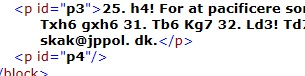
\includegraphics[scale=1.0]{figures/XmlIssue3}
	\caption{Excerpt of the XML file containing the data from article e410559d.}
	\label{XmlIssue3}
\end{figure}

\begin{figure}
	\centering
	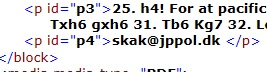
\includegraphics[scale=1.0]{figures/XmlIssue4}
	\caption{Excerpt of the XML file containing the data from article e410551d.}
	\label{XmlIssue4}
\end{figure}

Looking down the list of results there is a few interesting comparisons that have some scores, that makes it worth checking them out. The first of these we will look into is the comparison of articles \textit{e410557c} and \textit{e4105345}. This comparison scores relatively low with the Cosine algorithm, yet the LCS scores is pretty high (especially for the shortest article). The scores have been listed in table ~\ref{JPPOLPartialMatch}. We can also see the effect of having compared the length of the longest common substring with both the shortest and longest articles. No doubt that 38\% is a significant amount to have in common, but the 55\% really makes the score stand out. So what does this tell us? 

\begin{table}
\begin{center}
	\begin{tabular}{l | r}
	Ids & e410557c / e4105345\\ \hline
	Cosine & 0.407671899\\ \hline
	Basic LCS & 0.191534385\\ \hline
	LCS (long article) & 0.38342151\\ \hline
	LCS (short article) & 0.55743587\\ \hline
	Long article length & 2835\\ \hline
	Short article length & 1950\\ \hline	
	\end{tabular}
\end{center}
\caption{Scores for the 14th article comparison when comparing JP and POL sources (File: JPPOL.xlsx).}
\label{JPPOLPartialMatch}
\end{table}

First we will take a look on the LCS plot to try and get a visual indication of what could be going on. Figure ~\ref{ParticlaMatch} shows an excerpt of the LCS plot, the full plot is rather large, and would not fit in a single view in Excel. We will however not find any substrings with a length that fulfils the threshold outside the figure. The plot shows us that we have two articles that have quite a lot in common. Again we see issues with white spaces and also there are a few words words that breaks the longest common substrings. Overall we can say that the substrings found is sufficient identical and long (the breaks in between the substrings are quite short and the overall length of the substrings combined is rather long) to talk about a duplication. They only share an excerpt. That being said we also have a lot of text in the two articles that does not match, the match is therefore only partial. It is now obvious that we need to further divide the term \textit{'Match'} into subgroups, and we will do so later. When looking at the plot and then looking at the scores, we get a further explanation of what the scores tell us. The relative low Cosine score is influenced in part by the fact that there is quite a bit of text that is not shared by the articles, but also by the fact that the articles are of differing lengths.

\begin{figure}
	\centering
	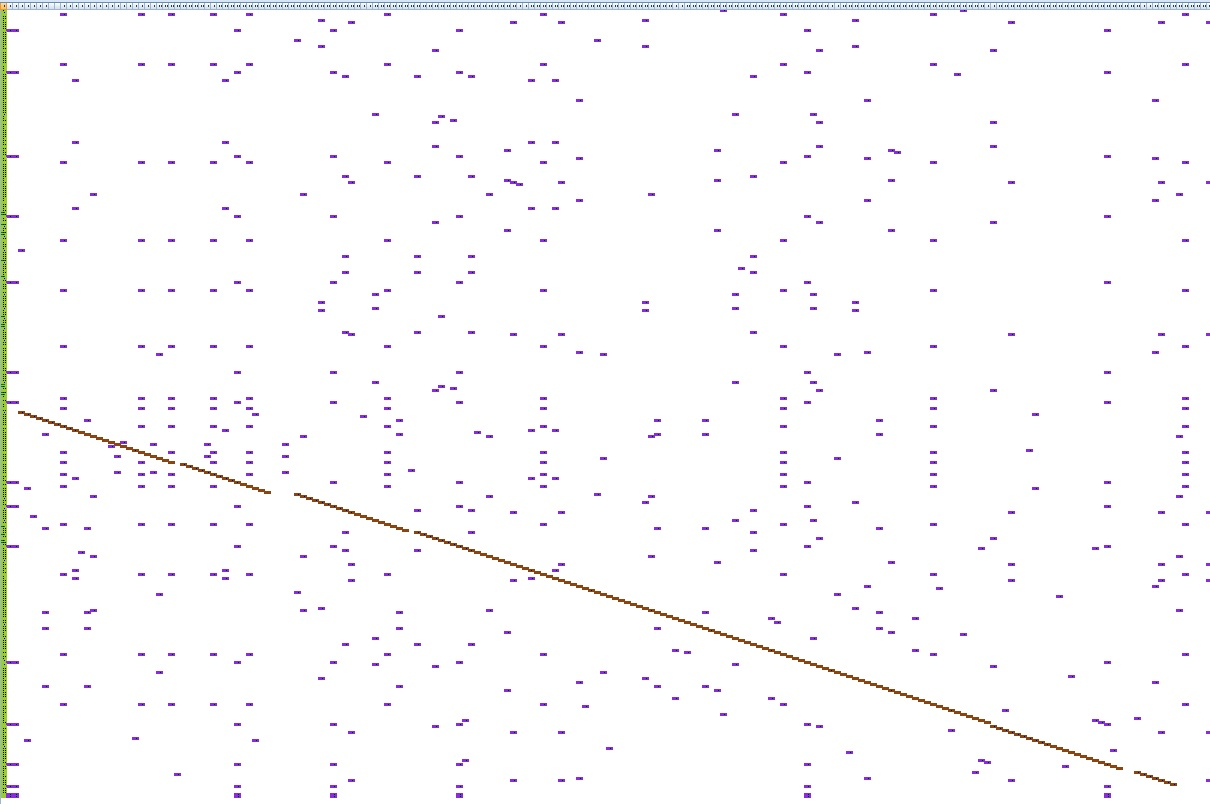
\includegraphics[scale=0.3]{figures/e410557c}
	\caption{LCS plot for the 14th article comparison in the set. The full plot is too big to be displayed in full in Excel, but the results can be seen in the file: e410557c-e4105345.xlsx.}
	\label{ParticlaMatch}
\end{figure}

The next comparison to be looked at is the 6th comparison (article Ids \textit{e410549c} and \textit{e4105515}). Here we have a fairly high Cosine score, but LCS scores are really low. The article lengths is fairly long, so we know it is articles that have some real content. The scores can be seen in table ~\ref{JPPOLSameContent}. Judging from the Cosine score, the articles have quite a bit in common, however the LCS score tells us that what ever they do have in common, is not expressed in sentences as such (we barely have any substrings in common). Once again we turn to the trusted to LCS plot to try and get an overview of what is going on.

\begin{table}
\begin{center}
	\begin{tabular}{l | r}
	Ids & e410549c / e4105515\\ \hline
	Cosine & 0.533468902\\ \hline
	Basic LCS & 0.0138186\\ \hline
	LCS (long article) & 0.013357899\\ \hline
	LCS (short article) & 0,017251637\\ \hline
	Long article length & 2171\\ \hline
	Short article length & 1681\\ \hline	
	\end{tabular}
\end{center}
\caption{Scores for the 6th article comparison when comparing JP and POL sources (File: JPPOL.xlsx).}
\label{JPPOLSameContent}
\end{table}

\begin{figure}
	\centering
	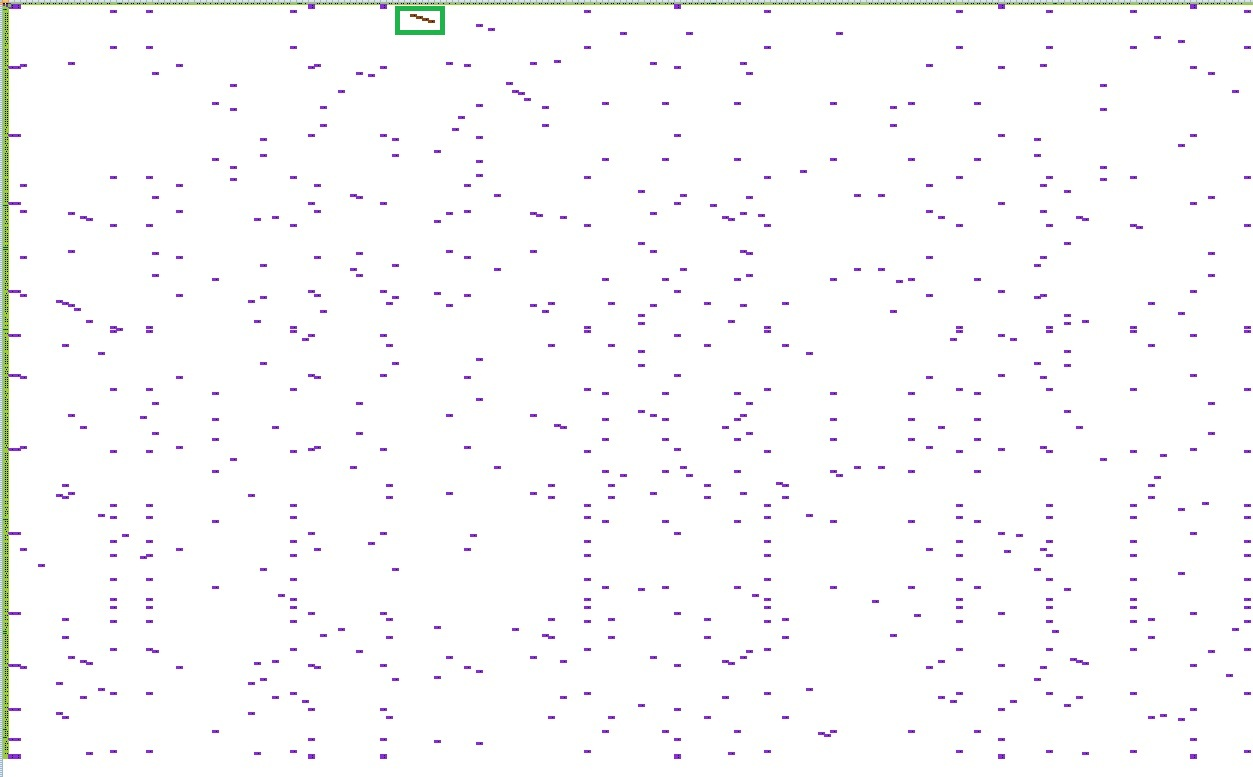
\includegraphics[scale=0.3]{figures/e410549c}
	\caption{LCS plot for the 6th article comparison in the set. The full plot is too big to be displayed in full in Excel, the full result can be seen in the file: e410549c-e4105515.xlsx. The only substring that is greater than the threshold have been marked in the green box.}
	\label{SameContent}
\end{figure}

In figure ~\ref{SameContent} we can see all substrings found, there is only one that is greater or equal to the threshold, it is marked in the green box. So the LCS plot does not tell us much about what is going on here, other than there truly is little in common in terms of substrings. We must then have a look at the article texts in order to see if we can figure out the reason for the relative high Cosine score. The two article's text can be found in appendix ~\ref{JPPOLSameContent1} and ~\ref{JPPOLSameContent2}. When reading the articles, it is clear that the articles is about the same topic (Brazilian footballer Carlos Bledorn Verri ('Dunga')), but are written in two different ways. If this started out with being a duplicate it has been obfuscated heavily, and it would be impossible to tell if that would be the reason. We can however say that the article have the same content, topic wise. A high (or relative high) Cosine score combined with a low LCS score, can then indicate that the article comparison are about the same topic, but without much other relation. This is something that we need to consider, and will get back to later.

\subsubsection{Low Scoring Comparison}
Finally for these sources an interesting case was found, when lowering the Cosine threshold to 0.1 (the results can be seen in the file: JYPPOL.xlsx). A comparison with the following scores was found ~\ref{JPPOLLowScoreMatch}. Both the Cosine and the LCS score for the longest article are really low. However looking at the LCS score for the short article a score of around 30\% is indicated. This would be a substantial part of the article that actually match the other article.

\begin{table}
\begin{center}
	\begin{tabular}{l | r}
	Ids & e41055d0 / e4105462\\ \hline
	Cosine & 0.105226949\\ \hline
	Basic LCS & 0,05952381\\ \hline
	LCS (long article) & 0,05952381\\ \hline
	LCS (short article) & 0,303030312\\ \hline
	Long article length & 168\\ \hline
	Short article length & 33\\ \hline	
	\end{tabular}
\end{center}
\caption{Scores for a low scoring (Cosine) comparison, with some interesting scores none the less. (File: JYPPOL.xlsx).}
\label{JPPOLLowScoreMatch}
\end{table}

When looking at the length of the articles, we can see that they are in fact quite short, the shortest being really short, only 33 characters long. This article will probably have very little interesting text (could be a breaking news article). Taking a look at the LCS plot helps to shed some light on the situation.

\begin{figure}
	\centering
	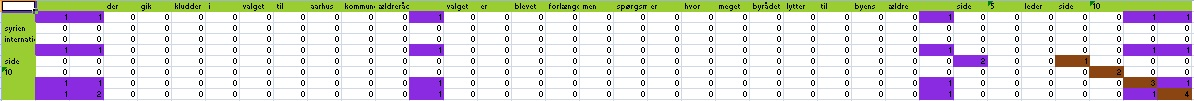
\includegraphics[scale=0.38]{figures/LengthIssue}
	\caption{LCS plot showing two very short articles being compared. This shows us an issue that can occur between the LCS score and the length of an article.}
	\label{LengthIssue}
\end{figure}

When looking at figure ~\ref{LengthIssue} we can see that the substring the two articles have in common are at the very end and is composed of the following: 
\begin{quote}
"side 10 \textvisiblespace \textvisiblespace"
\end{quote}

The short article (the word article used loosely here) does not contain any sort of informative text, other than a reference to the main article, and in such happened to have a very short substring in common with the other article. The substring just makes it to the threshold to be included, and one could consider from this to raise the threshold, but more testing into how inaccurate the results are from the current threshold is needed in order to see the overall impact of the threshold. But the length of the substring relative to the length of the article was enough to produce a substring that was just over 30\% of the article's length. So once again we must be aware of the length of the article, and this time also in combination with the LCS score. We must then ask the question is this a duplicate? To say it is not a match, is perhaps wrongful, but the contents of the short article would not really justify calling them a match. Later on we will try and look into how we can classify articles (in match groups) to giver a better indication of how well they match each other.

This example does show us, that interesting cases can be found in the comparisons that scores very low on the Cosine, but can still be a valid match (to some extend). In a future implementation, one should consider also looking into the low scoring comparisons.

\subsection{JV and FL Comparion}
In the following section, the article comparisons made from the sources JV and FL are being looked at. The file containing the results of this comparison is called JV-Lemvig.xlsx. A lot of the findings in this comparison will be similar to what was shown in the previous sections. We will therefore only look into results that brings something new to the table.

As there are many, many more comparisons in this set, the graph displaying the scores is incredible dense, and as it would be needed to scale it down, in order to make it fit the rapport, it would become nothing but a blur, so it will be left out of the chapter, the figure is instead found in appendix ~\ref{D3}.

The overall image of figure ~\ref{D3} is somewhat different from what we saw when comparing JP an POL. We are now seeing a lot of comparisons that looks to be matches, scoring high with both the Cosine and LCS algorithms. Now we are even seeing LCS scores that are greater than 1.0.

To look into why that is a closer inspection of the comparison seen in table ~\ref{JVFL100} is made.

\begin{table}
\begin{center}
	\begin{tabular}{l | r}
	Ids & e410c8b3 / e410c8c2\\ \hline
	Cosine & 0.929463029\\ \hline
	Basic LCS & 0.62894249\\ \hline
	LCS (long article) & 0.99072355\\ \hline
	LCS (short article) & 1,575221181\\ \hline
	Long article length & 539\\ \hline
	Short article length & 339\\ \hline	
	\end{tabular}
\end{center}
\caption{Scores for a low scoring (Cosine) comparison, with some interesting scores none the less. (File: JYPPOL.xlsx).}
\label{JVFL100}
\end{table}

The very high Cosine score indicates that a match has been found. Looking at the LCS scores, in particular the score for the shortest article, it is clear that the two article have a lot in common as the score indicates that the article shares 158\% of it's length with the other article. The articles are relative short, but not as short as to consider them having no "valuable" content. Again we turn to the trusted LCS plot to get a visual representation of the score.

\begin{figure}
	\centering
	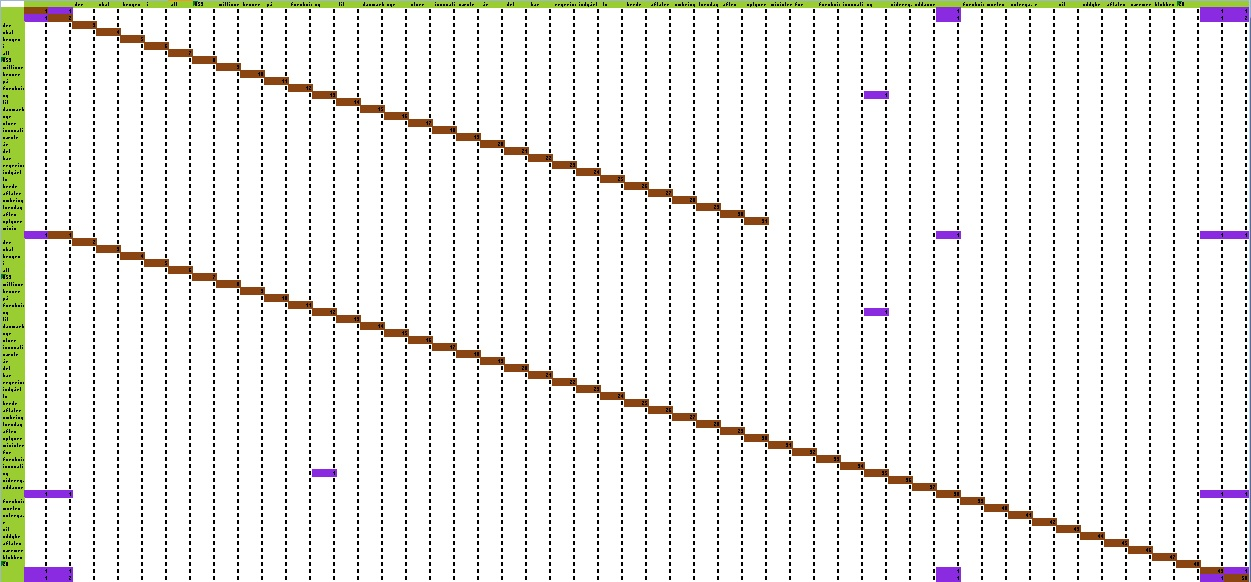
\includegraphics[scale=0.35]{figures/Over}
	\caption{LCS plotting showing what happens when text is repeated in the articles, we get an LCS score over 1.0.}
	\label{Over100}
\end{figure}

The plot in figure ~\ref{Over100} shows that we have two substrings of substantial length. When the substrings are placed in ways that they overlap in either direction, it means that text is repeated. This will often be the case when having a sub headline that are in turn repeated in the body text of the article (although it can also be a random collection of words, which all the purple squares shows). The text of the two articles can be found in appendix ~\ref{JVFLMatch1} and ~\ref{JVFLMatch2}. As it can be read from ~\ref{JVFLMatch2}, it has a lot of text repeated for some reason. This is the reason that the article scores more than 1.0 in the Cosine score. This result is not wrong per say, it just indicates that we have a lot of text in common in the articles being compared.

\section{Weighing the Scores}
In the previous sections we became aware that we need to do some amount of evaluation of various factors when determining if two articles are duplications. We need to take into account the length in combination with the scores, but also the scores in relation to each other. These factors all help us decide if we are looking at duplicates or not. In this section we will look into these factors and apply them to our comparisons.

In combination the two sets of scores (Cosine and both of the LCS scores) can draw us a more detailed picture, one that to a higher degree of confidence call tell about any relations between two articles. To try and break scores into something that is able to be defined, the following enums have been created, and called \textit{'Match Groups'}:

\begin{itemize}
\item \textbf{Match:} The comparison is to a high degree a perfect match, meaning that the two articles being compared have a lot of text in common, scores high with the algorithms and is somewhat similar in length.
\item \textbf{Partial Match:} This label would be a applied to a comparison, where only parts of the articles are shared, or that one article is a good deal shorter than the other, but scores highly in LCS. It would be considered an article excerpt.
\item \textbf{Same Content:} For comparisons with relative high Cosine scores, but somewhat low LCS scores, we can sometimes talk about the articles deal with the same topic, but without sharing much text. 
\item \textbf{Low Score Match:} Applying this label to a comparison would indicate that either one or both article are very short in length, can have a relative high Cosine score, but will have a high LCS score. It will indicate that the comparison most have a lot in common, but will maybe not contain much article text of much value.
\item \textbf{No Match:} When both algorithms scores low for a comparison, there is grounds to dismiss the comparison as a match. The articles will not have many sentences or special words in common.
\end{itemize}

The need for these match groups became obvious in the previous sections when we started to see comparisons that had a fairly high amount of text in common, but not enough to fully qualify as a duplicate.

The following table was created in order to try and give some weight to the scores. This could then be used in the program for score evaluation. The weight would be a factor that could be multiplied to the scores the algorithms produced in order to emphasize the result. These score weightings is based of tests that was done during the project.

\begin{table}
\begin{center}
	\begin{tabular}{l | c | c | c | c | c | c | c | c | c | c | r}
		    & 0.0 & 0.1 & 0.2 & 0.3 & 0.4 & 0.5 & 0.6 & 0.7 & 0.8 & 0.9 & 1.0\\ \hline
		0.0 & 0.01 & 0.01 & 0.01 & 0.01 & 0.01 & 0.01 & 0.01 & 0.01 & 0.01 & 0.01 & 0.01\\ \hline
		0.1 & 0.01 & 0.01 & 0.01 & 0.01 & 0.01 & 0.01 & 0.05 & 0.2 & 0.4 & 0.6 & 0.8\\ \hline
		0.2 & 0.01 & 0.01 & 0.05 & 0.1 & 0.1 & 0.1 & 0.3 & 0.5 & 0.6 & 0.8 & 0.85\\ \hline
		0.3 & 0.01 & 0.05 & 0.1 & 0.1 & 0.1 & 0.2 & 0.4 & 0.55 & 0.7 & 0.85 & 0.9\\ \hline
		0.4 & 0.01 & 0.05 & 0.1 & 0.1 & 0.1 & 0.2 & 0.4 & 0.6 & 0.75 & 0.85 & 0.95\\ \hline
		0.5 & 0.01 & 0.05 & 0.1 & 0.2 & 0.3 & 0.4 & 0.5 & 0.65 & 0.8 & 0.9 & 1.0\\ \hline
		0.6 & 0.01 & 0.07 & 0.1 & 0.2 & 0.4 & 0.5 & 0.6 & 0.7 & 0.85 & 0.9 & 1.0\\ \hline
		0.7 & 0.01 & 0.1 & 0.2 & 0.4 & 0.4 & 0.5 & 0.7 & 0.8 & 0.9 & 1.0 & 1.0\\ \hline
		0.8 & 0.01 & 0.1 & 0.4 & 0.6 & 0.7 & 0.8 & 0.8 & 0.9 & 1.0 & 1.0 & 1.0\\ \hline
		0.9 & 0.01 & 0.1 & 0.7 & 0.7 & 0.8 & 0.8 & 0.9 & 1.0 & 1.0 & 1.0 & 1.0\\ \hline
		1.0 & 0.05 & 0.2 & 0.8 & 0.8 & 0.9 & 0.9 & 1.0 & 1.0 & 1.0 & 1.0 & 1.0\\ \hline
	\end{tabular}
\end{center}
\caption{Score weights. The cosine score is the top most row and LCS score is the leftmost x axis. The weights indicates to what extend that articles have something in common. A low score would mean that the combination of Cosine and LCS score indicates that there is a low chance of any relation between the articles, a high score would mean the opposite. (File: Score Weight.xlsx)} \label{ScoreWeights}
\end{table}

The table ~\ref{ScoreWeights} would be an immediate indication as to how related two articles are, but we do also need to take another parameter into account, this being the length of the articles. A perfect match comparison would occur when two articles of the same length (roughly) and scoring close to 1.0 in both algorithms, but if two articles have a big difference in length that could affect the algorithm scores in a way that might not apply the right label when placing a comparison in a match group (as seen in figure ~\ref{LengthIssue}). The following enums was created to try and categorize articles by their length (table ~\ref{enums}).

\begin{table}
\begin{center}
	\begin{tabular}{l | c}
	Very Short & x < 300\\ \hline
	Short & x $\geq$ 300 $\bigwedge$ x < 500\\ \hline
	Medium & x $\geq$ 500 $\bigwedge$ x < 800\\ \hline
	Long & x $\geq$ 800 $\bigwedge$ x < 1200\\ \hline
	Very Long & x $\geq$ 1200\\ \hline
	\end{tabular}
\end{center}
\caption{Enums describing article length. X is the length of the article in characters and the values it is being compared with is the article length threshold for the various enums.}
	\label{enums}
\end{table}

\subsection{Applying the Score Weight}
Applying the weighing to the scores would only make sense if applied to the LCS score. The Cosine score is hard to alter in any meaningful way as it relates solely to the overall content matching. The LCS score can however become more useful if adjusted in accordance with the parameters discussed earlier. In the implementation only the LCS score based off the shortest article would be adjusted. This is because that this score would fluctuate more than the longer relative to it's length.

First off the article would be scored as normal. Once the post processing of the results would commence, all articles would get the enum describing their length. Then based of their length enums several methods was created to evaluate the LCS score based of the length and all of the comparisons scores. These methods was modelled in relation to table ~\ref{ScoreWeights}. The way it was modelled was to try and generate a lot of "buttons" that could be turned for many different cases of scores.

\lstset{style=sharpc}
\begin{lstlisting}[caption=Part of the method for applying LCS score weight, captionpos=b]
 class CalculateArticleScoreWeight
    {
        public float VeryShortVeryShort(float maxScore,
         float minScore, float shortArticleLength,
          float longArticleLength)
        {
            float factor = maxScore/minScore;
            if (shortArticleLength < 100 &&
             longArticleLength < 100)
            {
                if (factor > 0.8F && minScore > 0.7F)
                    return 1.0F;
                if (factor > 0.8F && minScore < 0.7F)
                    return 0.5F;
                return 0.1F;
            }

            if (shortArticleLength < 100 &&
             longArticleLength > 100)
            {
                if (factor > 0.8F && minScore > 0.6F)
                    return 1.0F;
                return 0.5F;
            }

            if (shortArticleLength > 100)
            {
                if (factor > 0.7F && minScore > 0.6F)
                    return 1.0F;
                return 0.6F;
            }
          }

\end{lstlisting}

<BESKRIV HVORDAN MATCHING GROUP BLEV TILSKREVET- KODE UDDRAG!!>



								%Chapter 6, Evaluation
\appendix	
\chapter{Test Diagrams}

Examples of comparing two articles with LCS. More files can be found in the electronic appendixes.

\begin{sidewaysfigure}
	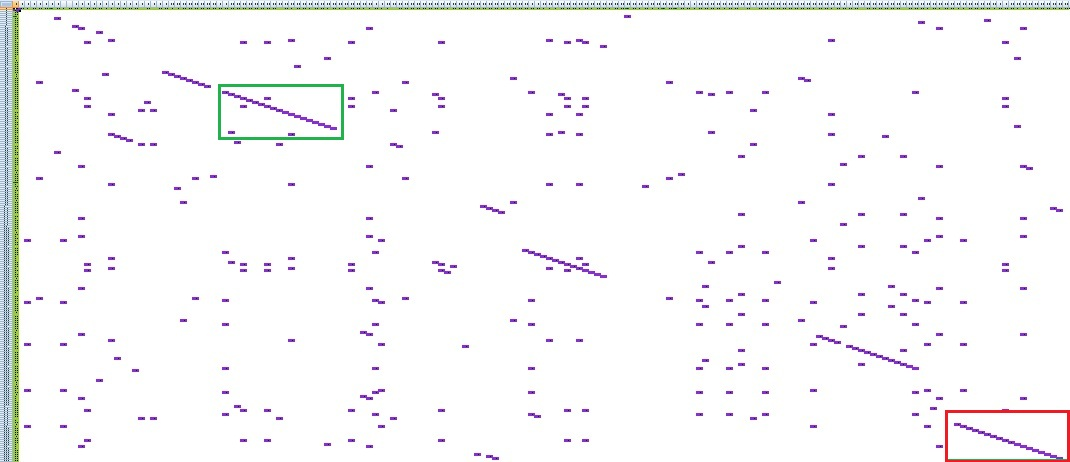
\includegraphics[scale=0.65]{figures/LcsExample}
	\caption{Diagram showing the result of two article being compared by using LCS.}
\end{sidewaysfigure}

\begin{sidewaysfigure}
	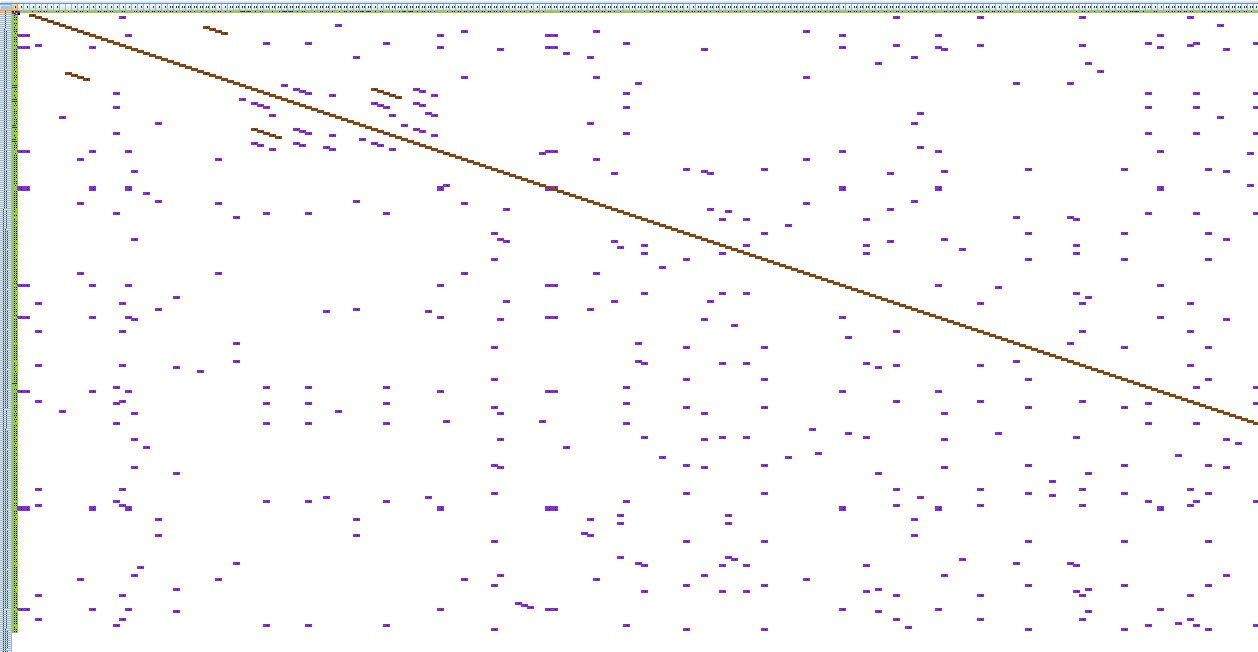
\includegraphics[scale=0.5]{figures/PerfectMatch}
	\caption{Diagram showing part of the result from running LCS on two articles that are almost a perfect match.}
\end{sidewaysfigure}

\begin{sidewaysfigure}
	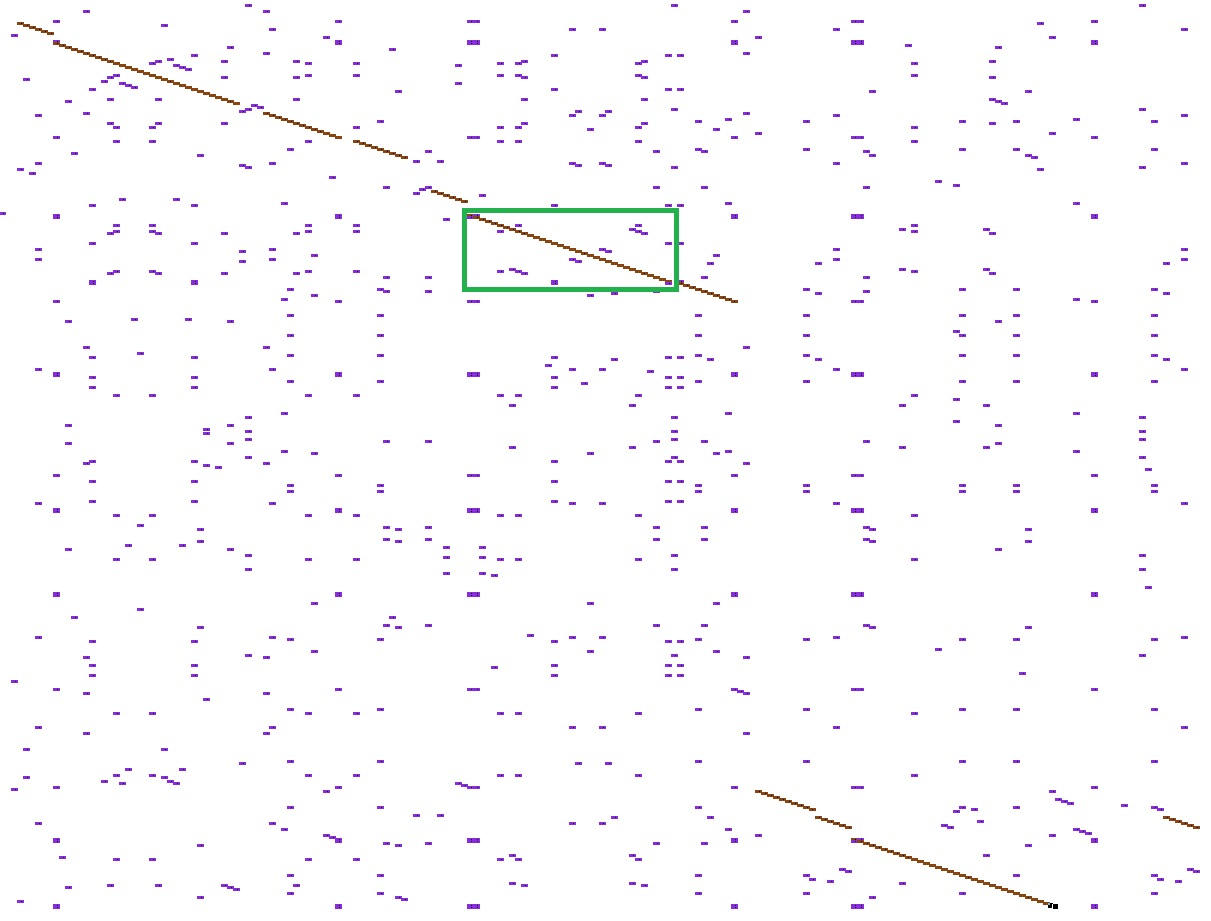
\includegraphics[scale=0.5]{figures/SubstringCollection}
	\caption{Diagram showing part of the result of running LCS on two articles and marking up all substrings with a length larger than three words.}
	\end{sidewaysfigure}                                 %Appendix A
\chapter{Article Content}
\section{Danfoss fastholder stabil forretning}
\label{Levmig1:text}
	Termostatkæmpen Danfoss holder sit indtjeningsniveau, mens omsætningen falder en smule.
	Ingen store dramaer i Danfoss.
	Det kunne være overskriften på selskabets regnskab for årets første ni måneder. Omsætningen falder en smule fra til 25.528 mio. kroner i år mod 25.985 mio. kroner i samme periode sidste år, mens indtjeningen lander på 2.938 mio. kroner i år mod 2.952 mio. kroner sidste år.
	Med andre ord en stabil forretning uden overraskelser, og det er koncernchef Niels B. Christiansen tilfreds med.
	»Takket være vores strategiske fokus på en stærk kerneforretning er vi i stand til at opveje både et kollapset europæisk solcellemarked og faldende valutakurser. Det er tilfredsstillende, at vi har formået at tilpasse os og levere så stærkt et resultat trods en generelt lav markedsvækst,« siger han.
	Selskabet anfører samtidig, at korrigeret for valutaeffekt er Danfoss' samlede omsætning på sidste års niveau.
	Det europæiske solcellekollaps har ellers ramt Danfoss hårdt, da selskabet producerer invertere til solcelleanlæg. Og solcellemarkedet var blandt de direkte årsager til, at Danfoss for tre måneder siden skar ned og fyrede 69 medarbejdere i Danmark.
	Den største vækst oplever Danfoss i Rusland og Brasilien, mens det kinesiske marked følger med i lavere tempo. Generelt forventer selskabet dog, at det globale marked vil være præget af lav vækst »et stykke tid endnu«. Og det åbner op for flere opkøb udover de seneste køb af Danfoss Turbocor og de sidste aktier i Sauer-Danfoss.
	»Derfor kigger vi meget på, om vi kan styrke forretningen gennem fokus på nye markeder og opkøb - såvel af nye teknologier som virksomheder. Vi har styrken til at kunne finansiere sådanne opkøb. Det giver en stor handlefrihed og mulighed for at forbedre Danfoss' position yderligere,« forklarer Niels B. Christiansen.
	For hele året venter Danfoss »beskeden vækst« i omsætning og indtjening.
	Danfoss' koncernchef Niels B. Christiansen venter "beskeden vækst" i år".

\section{Danfoss fastholder stabil forretning - w/o Stop Words}
\label{Lemvig1:textFiltered}
Termostatkæmpen Danfoss holder indtjeningsniveau, omsætningen falder smule. 	Ingen dramaer Danfoss. 	Det overskriften selskabets regnskab årets måneder. Omsætningen falder smule 25.528 mio. kroner 25.985 mio. kroner år, indtjeningen lander 2.938 mio. kroner 2.952 mio. kroner år. 	Med stabil forretning overraskelser, koncernchef Niels B. Christiansen tilfreds med. 	Takket strategiske fokus kerneforretning opveje kollapset solcellemarked faldende valutakurser. Det tilfredsstillende, formået tilpasse levere stærkt trods generelt markedsvækst, han. 	Selskabet anfører samtidig, korrigeret valutaeffekt Danfoss' samlede omsætning års niveau. 	Det europæiske solcellekollaps ellers ramt Danfoss hårdt, selskabet producerer invertere solcelleanlæg. Og solcellemarkedet blandt årsager til, Danfoss måneder skar fyrede 69 medarbejdere Danmark. 	Den største vækst oplever Danfoss Rusland Brasilien, kinesiske følger lavere tempo. Generelt forventer selskabet dog, globale præget vækst endnu. Og åbner opkøb udover seneste køb Danfoss Turbocor aktier Sauer-Danfoss. 	Derfor kigger på, styrke forretningen gennem fokus markeder opkøb - såvel teknologier virksomheder. Vi styrken finansiere sådanne opkøb. Det giver handlefrihed forbedre Danfoss' position yderligere, forklarer Niels B. Christiansen. 	For året venter Danfoss »beskeden vækst« omsætning indtjening. 	Danfoss' koncernchef Niels B. Christiansen venter beskeden vækst år. 							%Appendix containing article text
\chapter{Data Diagrams}

\begin{figure}
	\centering
	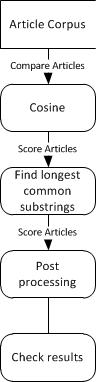
\includegraphics[scale=1.0]{figures/Dataflow}
	\caption{Diagram of the data flow in the system.}
\end{figure}

\begin{sidewaysfigure}
	\centering
	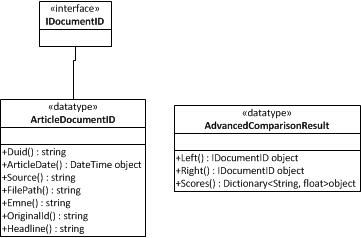
\includegraphics[scale=1.0]{figures/Datatypes}
	\caption{The general data types used in this project to store information about articles and their scores.}
\end{sidewaysfigure}						%Appendix containing diagrams about the dataflow
\chapter{Evaluation Diagrams}
This contains the diagrams used in the Evaluation chapter.

\begin{sidewaysfigure}
	\centering
	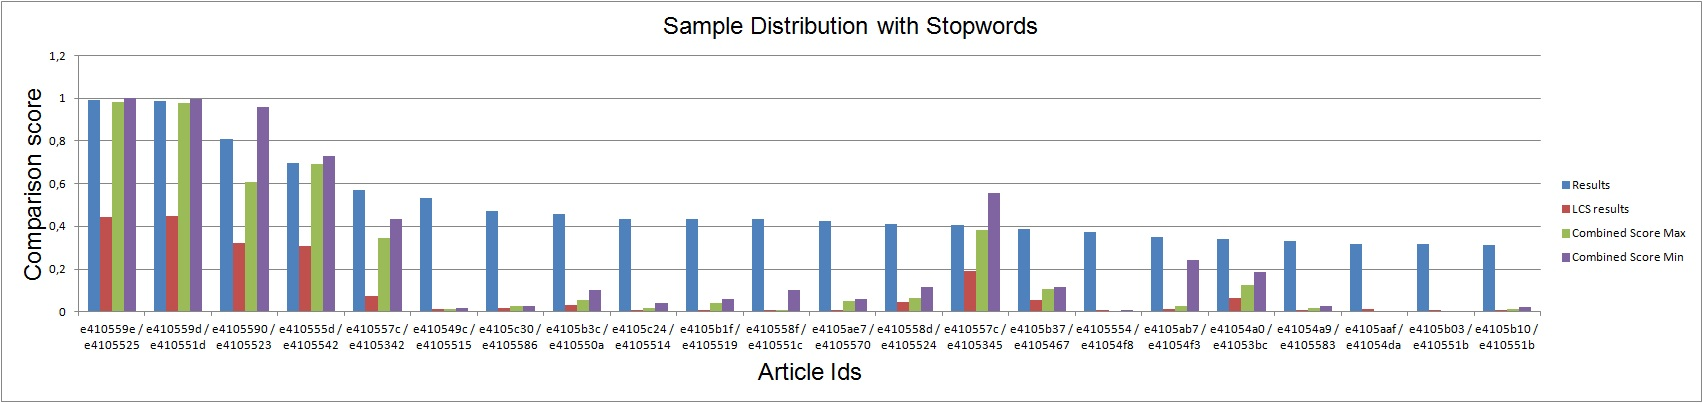
\includegraphics[scale=0.45]{figures/JPPOLScoreGraph}
	\label{D1}
\end{sidewaysfigure}						%Appendix containing digrams used in the evaluation
%-----------
% Backmatter
%-----------
\backmatter
\chaptermark{Bibliography}
\renewcommand{\sectionmark}[1]{\markright{#1}}
\sectionmark{Bibliography}
\addcontentsline{toc}{chapter}{Bibliography}        %Force addition of Bibliography to TOC
\bibliographystyle{alpha}                           %Use alpha codes for references
\bibliography{Refs}                          		%Bibliography file called
\end{document}
% % % EOF % % %